\documentclass[10pt]{beamer}

\usepackage{amsmath,amssymb}
\usepackage{zxjatype}
\usepackage[ipa]{zxjafont}
\usetheme[progressbar=frametitle]{metropolis}
\usepackage{tikz}
\usepackage{tikzsymbols}
\usepackage{appendixnumberbeamer}
\usepackage{minted}
\usepackage{url}
\usepackage{bm}

\usetikzlibrary{positioning}
\usefonttheme{professionalfonts}

\setminted[python]{frame=single}

% --- page number ---
\setbeamertemplate{footline}{%
	\raisebox{10pt}{\makebox[\paperwidth]{\hfill\makebox[7em]{\normalsize\texttt{\insertframenumber/\inserttotalframenumber}\hspace{1em}}}}%
}

% --- title logo ---
\newcommand{\myinsertlogo}[1]{%
\begin{tikzpicture}[overlay, remember picture]
    \node[above left=1cm and .8cm of current page.south east] {\includegraphics[width=2.25cm]{#1}};
\end{tikzpicture}}

% --- utils ---
\newcommand{\mymain}[1]{\textcolor{mLightBrown}{#1}}
\newcommand{\myaccent}[1]{\textcolor{mLightGreen}{#1}}
\newcommand{\red}[1]{\textcolor{red}{#1}}
\newcommand{\blue}[1]{\textcolor{blue}{#1}}

\title{Computer Vision in Python with OpenCV}
\date{February 3, 2019}
\author{Satoshi Murashige}
\institute{Mathematical Informatics Lab., NAIST}

\begin{document}
	\begin{frame}[plain]
		\maketitle
		\myinsertlogo{naist.pdf}
	\end{frame}
	\begin{frame}{Text books}
	    \begin{itemize}
	        \item A.\ Kaehler and G.\ Bradski,『詳解 OpenCV 3』, オライリー・ジャパン, 2018.
	        \item 原田達也,『画像認識 (機械学習プロフェッショナルシリーズ)』, 講談社, 2017.
	    \end{itemize}
	\end{frame}
	\begin{frame}{Table of Contents}
		\begin{enumerate}
		    \item はじめに
		    \item Numpy基礎
			\item 基本的な画像処理
				\begin{itemize}
					\item 1章:概要
					\item 2章:OpenCV入門
					\item 10章:フィルタとコンボリューション
				\end{itemize}
			\item 物体検出
				\begin{itemize}
					%\item 12章:画像解析
					\item 13章:ヒストグラムとテンプレートマッチング
					\item 14章:輪郭
				\end{itemize}
			\item 動画解析
				\begin{itemize}
					\item 15章:背景除去
					\item 16章:キーポイントと記述子
					\item 17章:トラッキング
				\end{itemize}
			\item 3次元復元
				\begin{itemize}
					\item 18章:カメラモデルとキャリブレーション
					\item 19章:射影変換と3次元ビジョン
				\end{itemize}
		\end{enumerate}
	\end{frame}
	
	\section{はじめに}

	\begin{frame}{サンプルコードについて}
		\begin{itemize}
			\item テキスト中のプログラムはすべてC++で書かれている
			\item 今回使用するコードはそれらをPython向けに書き直したもの
				\begin{itemize}
					\item 全部は書き直していない \Winkey[1.5]
					\item なるべくPythonicなスタイルにするのと説明の都合により機能が異なることがある
				\end{itemize}
            \item コード無しの解説や関数の紹介で終わってるところは補足のコードを追加してるので,
                テキストにないコードがいっぱいあるので注意
		\end{itemize}
	\end{frame}
	
	\begin{frame}[fragile]{前準備}
		\begin{itemize}
		    \item PythonをAnacondaでインストールする
		    \item OpenCVをインストールする
		        \begin{center}
		            \texttt{\$ conda install -c conda-forge opencv}
		        \end{center}
			\item サンプルコードのリポジトリをダウンロードする
				\begin{center}
					\url{https://github.com/eqs/opencv3-book-python.git}
				\end{center}
			\item 画像処理用の画像をダウンロードする
				\begin{itemize}
					\item \mymain{\texttt{cd}}コマンドで\mymain{\texttt{images}}に
						移動してから\mymain{\texttt{sh get\_images.sh}}を実行
				\end{itemize}
		\end{itemize}
	\end{frame}
	
	\begin{frame}{今日の目標}
	    \begin{center}
    	    動画からマウスの位置を追跡する画像処理を作る
    	    
	        \url{https://bit.ly/2GiMNPA}
	    \end{center}
	\end{frame}
	
	\begin{frame}{OpenCVを用いたコンピュータビジョンのタスクにPythonを\\使用するメリット・デメリット}
	
	    {\large Pythonを使用するメリット \red{\Smiley[1.5]}}
		\begin{itemize}
			\item コンパイル不要なのでTry \& Errorがしやすい
			\item 言語の使用難易度が低い(記述が簡潔・メモリ管理が楽)
			\item Python向けの強力な開発環境の恩恵を受けられる
			\item Pythonで書かれた他のモジュールとの組み合わせが容易になる
		\end{itemize}
		{\large Pythonを使用するデメリット \blue{\Sadey[1.5]}}
		\begin{itemize}
			\item 上手に書かないとめっちゃ遅くなる
			\item 上手に書いても最適化されたC++の速度には及ばない \\
				(リアルタイム性が求められなければ最低限の最適化でOK)
			\item 一部,C++でしか使えないモジュールがある
		\end{itemize}
		\note{
		    Pythonを使うと実行速度は下がるがコーディング時の生産性は上がる
		}
	\end{frame}

	\begin{frame}{画像処理プログラミングの環境の選択肢}
	    \begin{itemize}
	        \item 好きなエディタを使う (Vim, Atom, Visual Studio Code, ...)
	        \item Spyder IDE
	            \begin{itemize}
	                \item MATLABライクなPythonの統合開発環境
	                \item デスクトップアプリケーションとして動作
	            \end{itemize}
	        \item JupyterLab
	            \begin{itemize}
	                \item コード・図・ドキュメントを一元管理できるノートブックを編集できる統合開発環境
	                \item サーバとして動作し,ブラウザからアクセスして利用できる
	                \item Jupyter Notebookの機能拡張版
	            \end{itemize}
	    \end{itemize}
	\end{frame}
	
	\begin{frame}{Spyder IDE}
	    \begin{center}
	        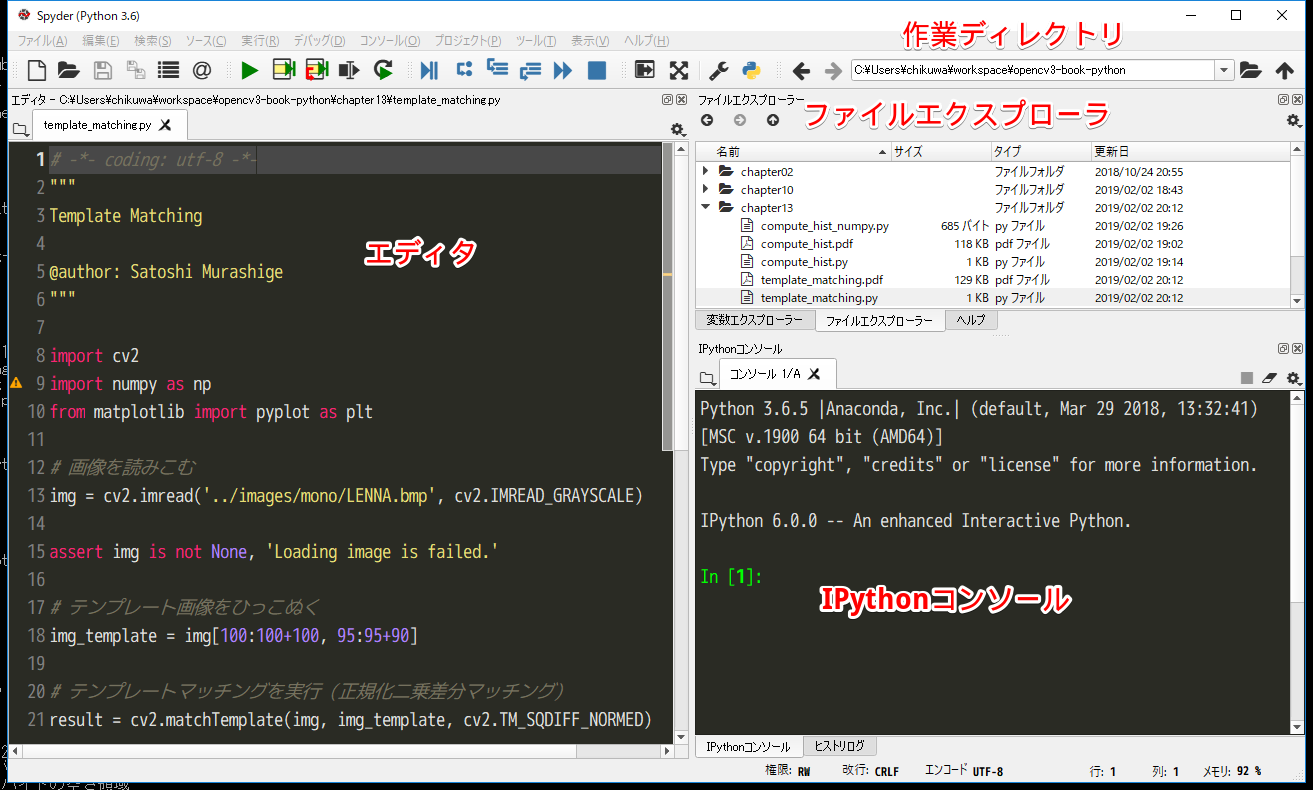
\includegraphics[width=\hsize]{figs/spyder.png}
	    \end{center}
	\end{frame}
	
	\begin{frame}{JupyterLab}
	    \begin{center}
	        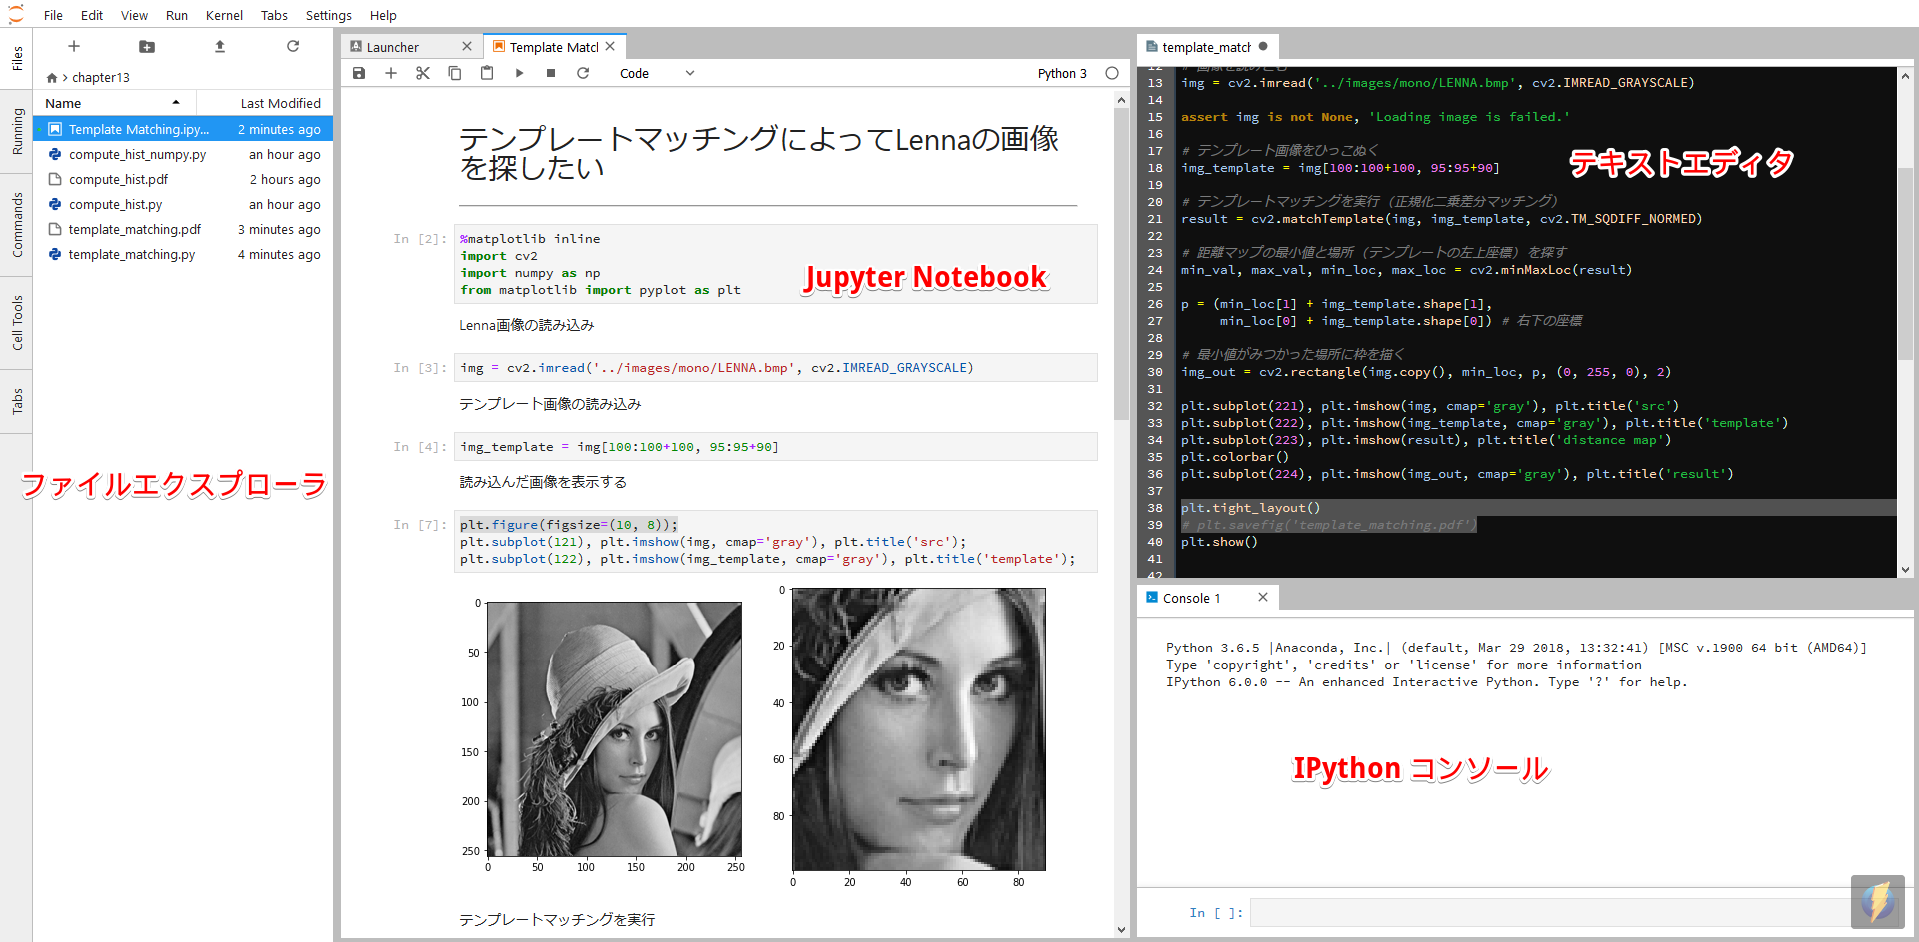
\includegraphics[width=\hsize]{figs/JupyterLab.png}
	    \end{center}
	\end{frame}
	
	\begin{frame}{なぜ環境が大事か?}
	    \begin{itemize}
            \item 開発環境に関する宗教戦争は不毛だしどうでもいい
                \begin{itemize}
                    \item e.g.\ Vim vs.\ Emacs
                \end{itemize}
            \item 作業内容に合わせて環境は選択すべし
            \item 画像処理のプログラミングはデータを見ながらTry and Errorのサイクルをひたすら回す作業が多いので,
                これに合致する環境を選択するのが望ましい
            \item ムラシゲがJupyterLabでよくやる開発体制
                \begin{itemize}
                    \item Jupyter Notebookで試行錯誤しながらアルゴリズムを作る
                    \item テキストエディタにコードをコピペ\&整形しながら単体のスクリプトとして体裁を整える
                    \item 関数の使い方を忘れたらヘルプを叩く
                    \item Numpy配列の形状操作の確認をコンソールでやる
                \end{itemize}
	    \end{itemize}
	\end{frame}
	
	\section{Numpy基礎}
	
	\begin{frame}{なんでNumpy?}
	    \begin{itemize}
	        \item OpenCV for Pythonでは,画像を扱うデータ構造としてNumpyが採用されている
	        \item 画像の特定のチャネルや部分画像の切り出し,プロット用のデータ整形など,扱い方を理解してないと困る
	    \end{itemize}
	\end{frame}
	
	\begin{frame}[fragile]{Numpy配列の基本:配列の定義と値の参照}
        \begin{itemize}
            \item モジュールのインポート
                \begin{minted}[fontsize=\scriptsize]{python}
import numpy as np # or import numpy
                \end{minted}
            \item 5つの整数を要素として持つ配列\texttt{a}を定義
                \begin{minted}[fontsize=\scriptsize]{python}
>>> a = np.array([100, 200, 300, 400, 500])
>>> # 等価なコード: a = np.arange(1, 5 + 1) * 100
                \end{minted}
            \item 配列\texttt{a}の中身を参照する
                \begin{minted}[fontsize=\scriptsize]{python}
>>> a[3]
400
>>> a[0]
100
                \end{minted}
	    \end{itemize}
	    \begin{center}
	        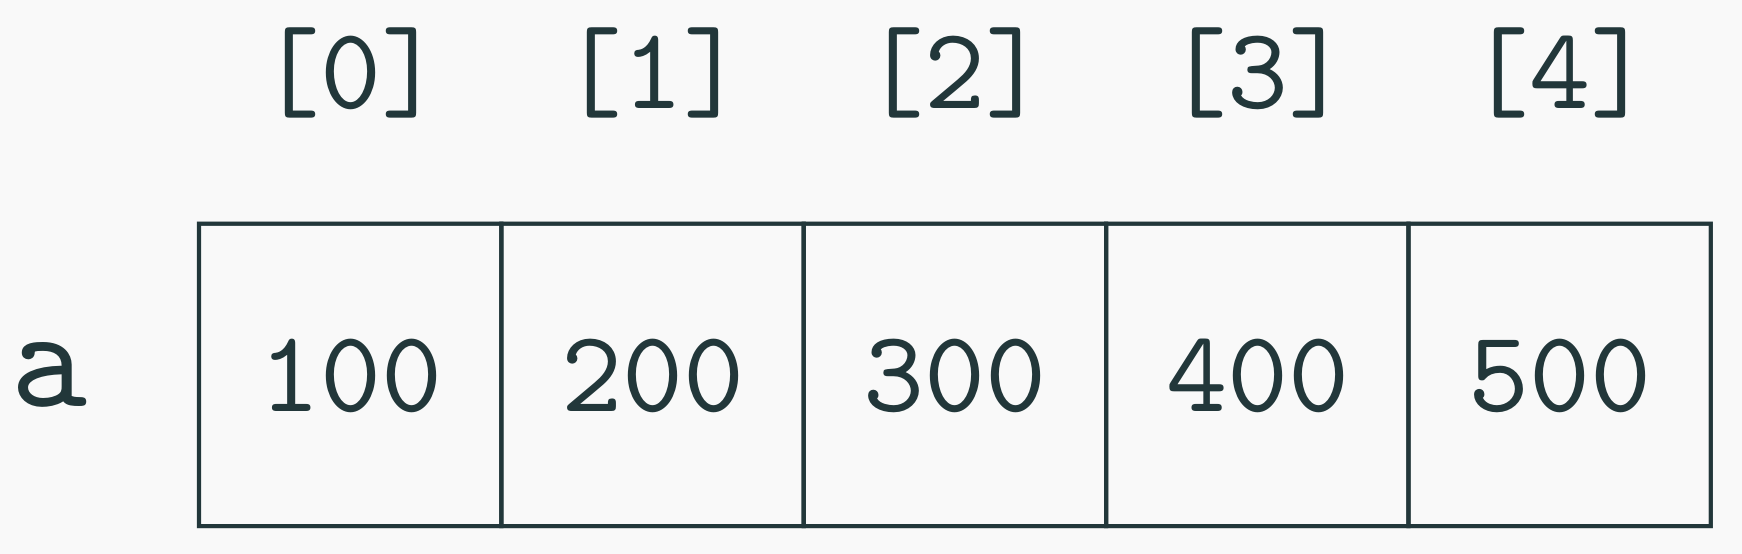
\includegraphics[width=0.5\hsize]{figs/numpy1.png}
	    \end{center}
	\end{frame}
	
    \begin{frame}[fragile]{Numpy配列の基本:部分配列を求める}
        \begin{columns}
            \begin{column}[c]{0.5\hsize}
                \begin{minted}[fontsize=\normalsize]{python}
>>> a[1:3]
[200, 300]

>>> a[0:4]
[100, 200, 300]

>>> a[2:]
[300, 400, 500]
                \end{minted}
            \end{column}
            \begin{column}[c]{0.5\hsize}
        	    \begin{center}
        	        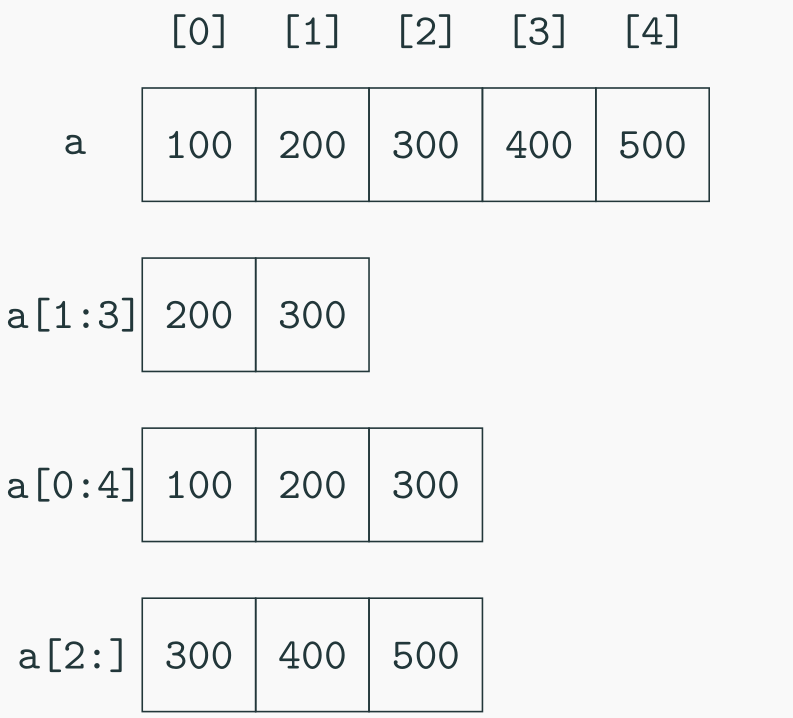
\includegraphics[width=\hsize]{figs/numpy2.png}
        	    \end{center}
            \end{column}
        \end{columns}
	\end{frame}
    
    \begin{frame}[fragile]{Numpy配列の基本:2次元配列}
        \begin{itemize}
            \item 2行3列の配列\texttt{a}を定義
                \begin{minted}[fontsize=\scriptsize]{python}
>>> a = np.array([100, 200, 300], [400, 500, 600])
>>> # 等価なコード: a = np.arange(1, 6 + 1).reshape((2, 3)) * 100
                \end{minted}
            \item 配列\texttt{a}の中身を参照する
                \begin{minted}[fontsize=\scriptsize]{python}
>>> a[0, 0]
100

>>> a[1, 2]
600

>>> a[0, 1]
200
                \end{minted}
	    \end{itemize}
	    \begin{center}
	        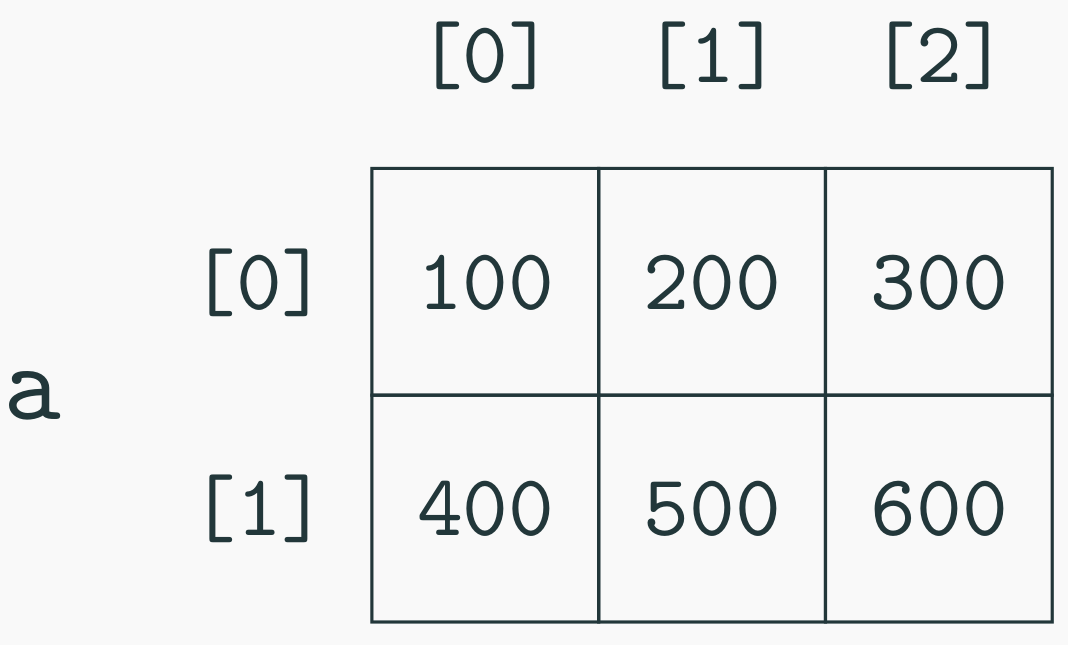
\includegraphics[width=0.35\hsize]{figs/numpy3.png}
	    \end{center}
	\end{frame}
    
    \begin{frame}[fragile]{Numpy配列の基本:2次元配列の部分配列を求める}
        \begin{minted}[fontsize=\normalsize]{python}
>>> a = np.arange(25).reshape((5, 5))
        \end{minted}
        \begin{center}
            \onslide*<1>{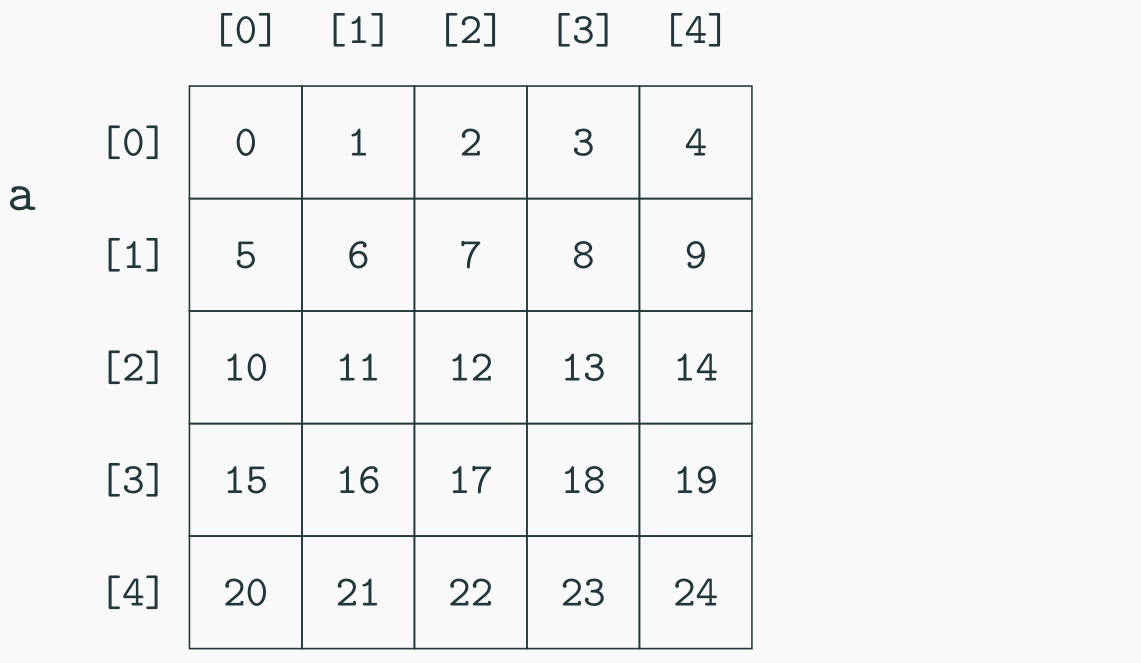
\includegraphics[width=0.85\hsize]{figs/numpy4_1.png}}%
            \onslide*<2>{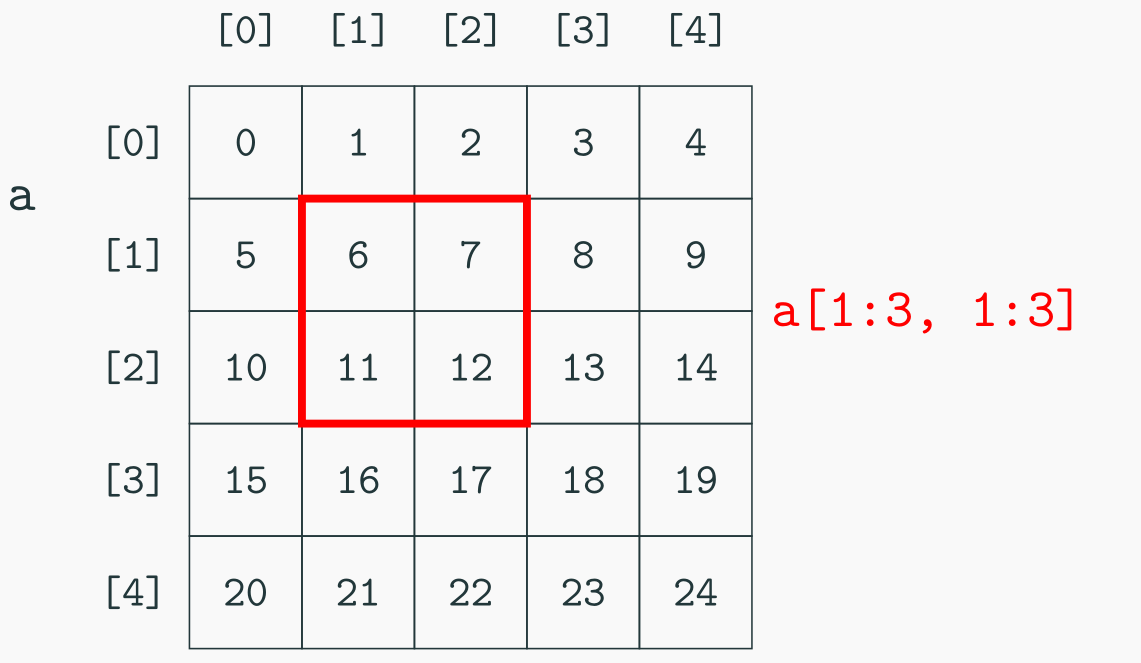
\includegraphics[width=0.85\hsize]{figs/numpy4_2.png}}%
            \onslide*<3>{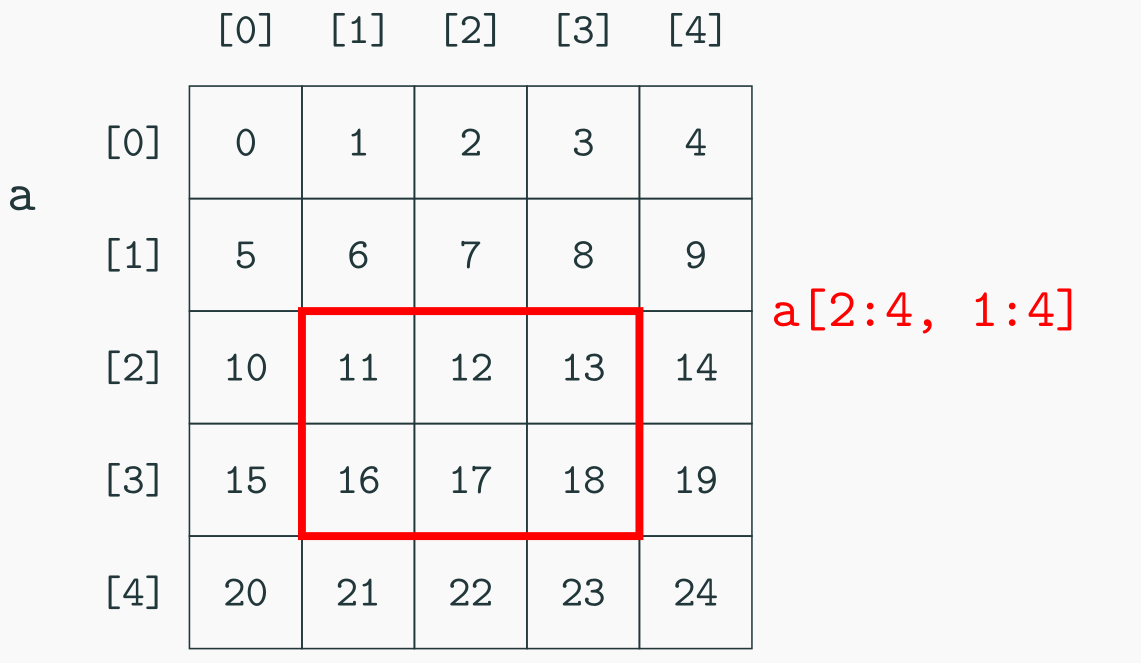
\includegraphics[width=0.85\hsize]{figs/numpy4_3.png}}%
            \onslide*<4>{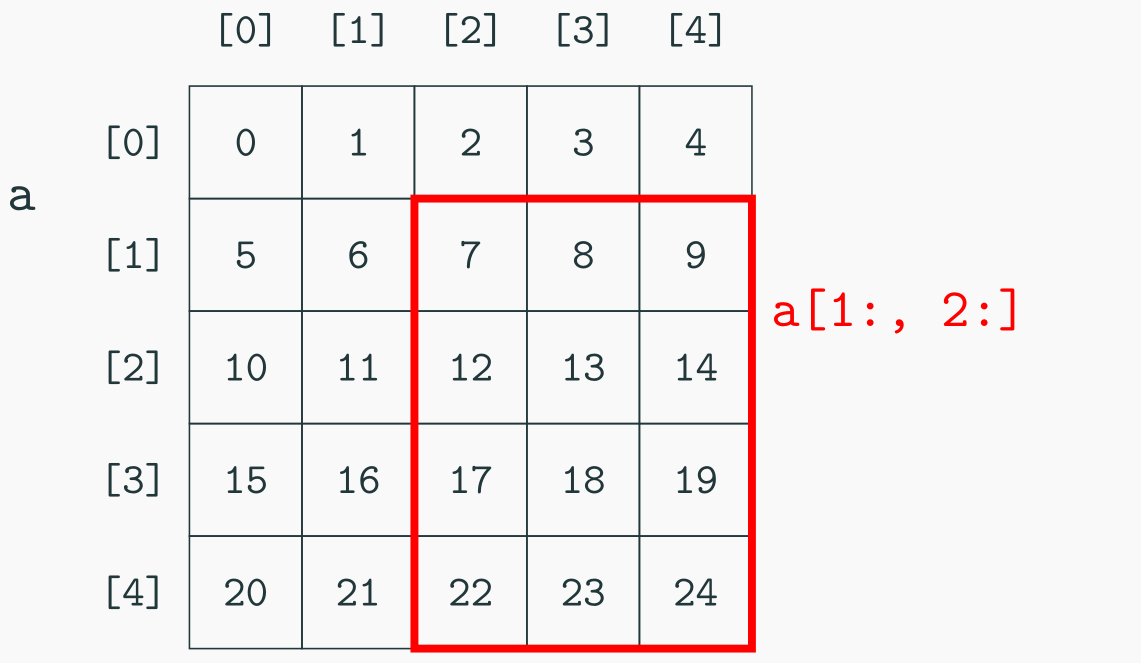
\includegraphics[width=0.85\hsize]{figs/numpy4_4.png}}%
            \onslide*<5>{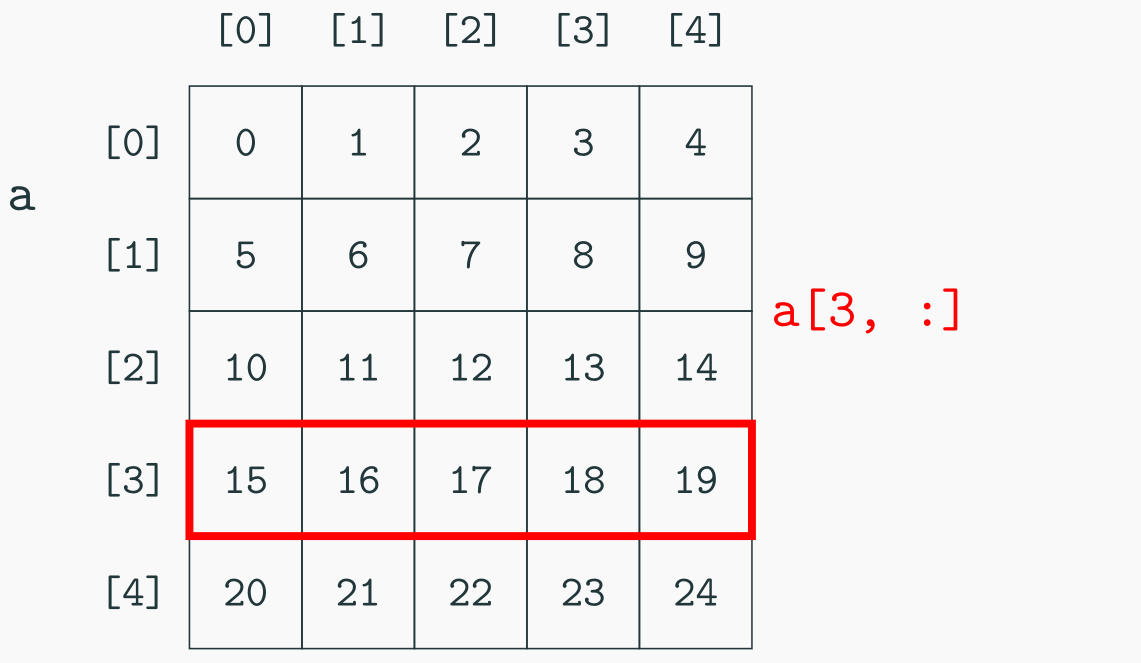
\includegraphics[width=0.85\hsize]{figs/numpy4_5.png}}%
            \onslide*<6>{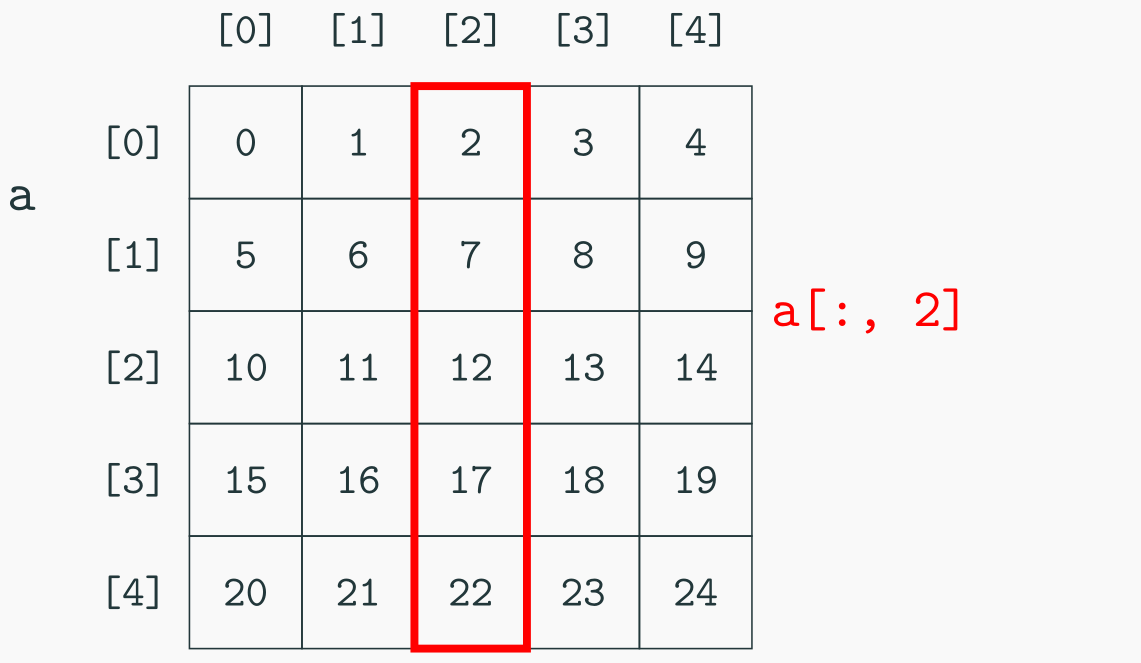
\includegraphics[width=0.85\hsize]{figs/numpy4_6.png}}%
        \end{center}
	\end{frame}
	
    \begin{frame}[fragile]{Numpy配列の基本:画像のチャネルをとってくる操作}
        \begin{minted}[fontsize=\scriptsize]{python}
# 横が640, 縦が480ピクセルのRGBカラー画像に見立てたダミー
>>> a = np.arange(480 * 640 * 3).reshape((480, 640, 3))

# チャネルの取り出し
>>> a[:, :, 0] # Rのチャネル
>>> a[:, :, 1] # Gのチャネル
>>> a[:, :, 2] # Bのチャネル
        \end{minted}
	\end{frame}
    
    \begin{frame}[fragile]{Numpy配列の基本:配列同士の演算}
        \begin{center}
            \onslide*<1>{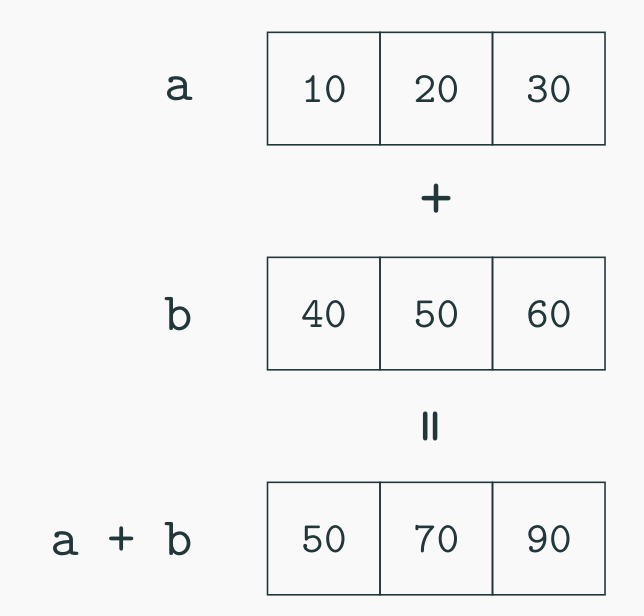
\includegraphics[width=0.6\hsize]{figs/numpy5_1.png}}%
            \onslide*<2>{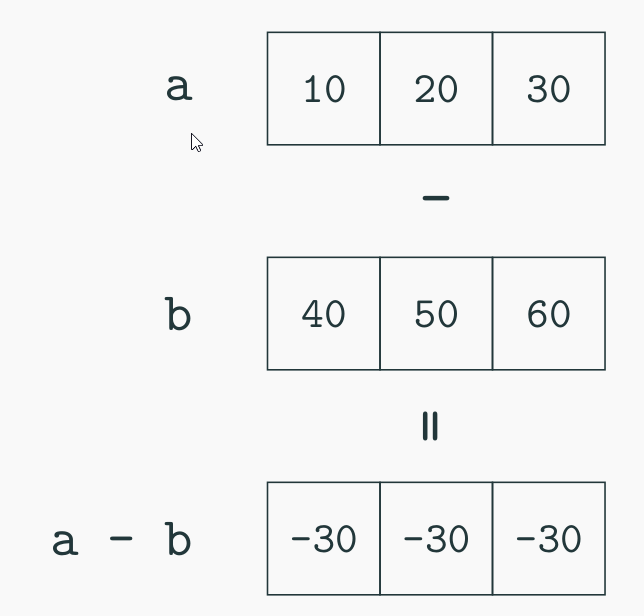
\includegraphics[width=0.6\hsize]{figs/numpy5_2.png}}%
            \onslide*<3>{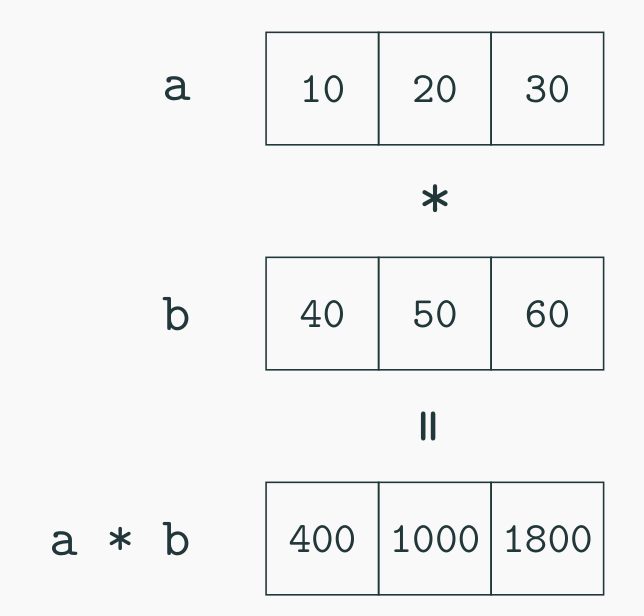
\includegraphics[width=0.6\hsize]{figs/numpy5_3.png}}%
            \onslide*<4>{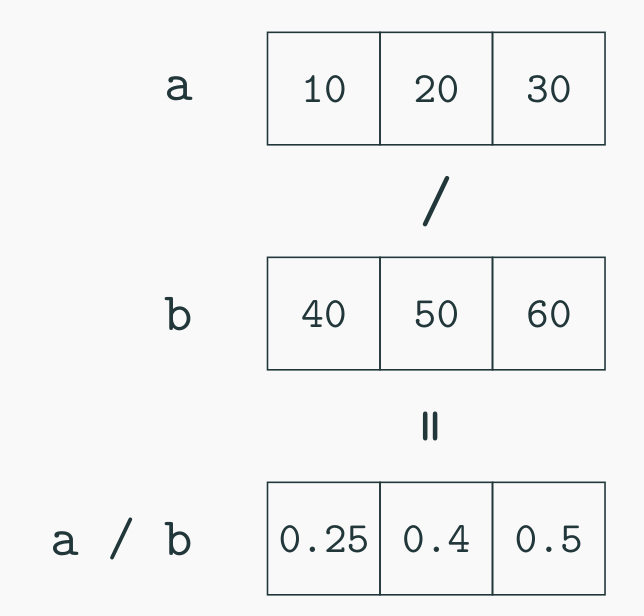
\includegraphics[width=0.6\hsize]{figs/numpy5_4.png}}%
        \end{center}
	\end{frame}
	
	\section{1章:概要}

	\begin{frame}{OpenCVとは何か?}
		\begin{itemize}
    	    \item 1999年にIntel社のGary Bradski (原著者のひとり) が立ち上げたオープンソースのコンピュータビジョンライブラリ
            \item OpenCVのゴールのひとつは,洗練されたビジョンアプリケーションをすばやく構築するのに役立つ使いやすいCVの基盤を提供すること
                \begin{itemize}
                    \item 画像処理に詳しい人がツール的に使う感じ.画像処理の知識が無いまま使うものではない
                \end{itemize}
		    \item ライブラリはC++で記述されているが,Python, Java, MATLAB向けのインタフェースがある
		        \begin{itemize}
		            \item C言語もサポートされていたが,現在はレガシーコード扱いになってるはず
		        \end{itemize}
            \item 機械学習や深層学習のライブラリも含まれている
		\end{itemize}
	    \note{
	        Cのコードを見かけたらブラウザバック推奨
	    }
	\end{frame}
	
	\begin{frame}{OpenCVを使うのは誰か?}
	    \begin{itemize}
            \item 用途
                \begin{itemize}
                    \item 工場の製品検査システム
                    \item 航空地図や市街地図のカメラキャリブレーションと画像結合
                    \item 無人機やロボットの視覚システム
                    \item 生物画像の自動解析(トラッキング,カウント,方向推定など)
                \end{itemize}
            \item OpenCVは商用製品を開発できるライセンスであり,
                オープンソース化は義務付けられていない
        \end{itemize}
	\end{frame}
	
	\begin{frame}{コンピュータビジョンとは何か?}
	    \begin{itemize}
	        \item 特定の目的のために,ディジタルカメラやビデオカメラからのデータを変換して
	            何らかの判断を行ったり別の表現にしたりすること
	            \begin{itemize}
	                \item 例1: 車載カメラの映像から,進行方向に人がいるか判断する
	                \item 例2: 顕微鏡画像にうつっている細胞の数を数える
	                \item 例3: カメラの映像から手ブレを補正した画像を作る
	            \end{itemize}
	        \item コンピュータにはヒトが持つ高度なセンサーも情報処理システムも無い
	            \begin{itemize}
	                \item カメラから得られた\mymain{数値のグリッド}から課題を解決する
	            \end{itemize}
	    \end{itemize}
	\end{frame}
	
	\begin{frame}{コンピュータビジョン:不良設定問題との闘いの日々}
	
	    {\large 襲い掛かる不良設定問題達\blue{\Xey[1.5]}}
        \begin{itemize}
	        \item 2次元画像から3次元シーンを復元する問題において,
    	        2次元画像として投影される3次元シーンは無限に存在する
	        \item カメラの熱雑音,レンズ歪み,照明のムラや画像圧縮などによるデータの劣化
	        \item 歩行者検出やりたいけど色々な服装の人がいる
        \end{itemize}
	    {\large コンピュータビジョンと向き合う際の基本方針\red{\Cooley[1.5]}}
        \begin{itemize}
            \item 目的に合わせた制約(ソフト的,ハード的)を入れることで問題を簡単化する
            \item 不要な一般化を避ける・解くべき問題のみに集中する
            \item 不良設定問題を見抜くのもスキル(白旗を揚げるのも選択肢)
        \end{itemize}
        
	\end{frame}
	
	\begin{frame}{OpenCVのオンラインドキュメント}
	    \begin{itemize}
	        \item 最新版 (4.0.0-pre) のチュートリアル
	            \begin{itemize}
	                \item \url{https://docs.opencv.org/master/d9/df8/tutorial_root.html}
	                \item C++, Java, Pythonでのコードが読める
	            \end{itemize}
	        \item イントロダクション
	            \begin{itemize}
	                \item \url{https://docs.opencv.org/master/df/d65/tutorial_table_of_content_introduction.html}
	                \item チュートリアルからさらに項目を厳選したもの
	                \item プラットフォームごとの環境構築の手順も含まれている
	            \end{itemize}
	        \item チートシート (C++, OpenCV 2.4用)
	            \begin{itemize}
	                \item \url{https://docs.opencv.org/3.0-last-rst/opencv_cheatsheet.pdf}
	                \item OpenCVのライブラリ全体を集約したチートシート
	                \item Python用ではないので,関数名のチェック用みたいな感じ
	                \item 印刷して壁に貼ろう
	            \end{itemize}
	    \end{itemize}
	\end{frame}
	
	\begin{frame}{OpenCVのリポジトリは\texttt{opencv}と\texttt{opencv\_contrib}に分かれている}
	    \begin{itemize}
	        \item \texttt{opencv}: OpenCVチームによって保守されている安定したコード
	        \item \texttt{opencv\_contrib}: コミュニティによって保守・開発されている最先端の手法のコード
	            \begin{itemize}
	                \item 深層学習,顔認識,RGB-D画像,Non-Photorealistic Rendering,Structure from Motion (SfM) 等
	            \end{itemize}
	    \end{itemize}
	\end{frame}
	
	\begin{frame}{OpenCV for Pythonの特徴}
	    \begin{itemize}
	        \item 画像を扱うデータ構造として,C++ではMatクラスを使うがPythonではNumpyを使う
	        \item Numpyの機能でOpenCVの関数を代替できることもある
	        \item \texttt{opencv\_contrib}のモジュールはPythonインタフェースが無いものもあるので注意
	    \end{itemize}
	\end{frame}
	
	\begin{frame}[fragile]{関数のドキュメントを読みたいとき}
	    \begin{itemize}
	        \item IPythonの場合
	            \begin{itemize}
	                \item 関数名の後ろに\texttt{?}をつけて実行 \\
	                \mint{python}|>>> cv2.getGaussianKernel?|
	            \end{itemize}
            \item Spyder IDEの場合
	            \begin{itemize}
	                \item 関数名にテキストのカーソルを合わせてから\texttt{Ctrl + I}
	                \item IPython同時に開くのもおk
	            \end{itemize}
	        \item Jupyter Notebook, JupyterLabの場合
	            \begin{itemize}
	                \item 関数名にテキストのカーソルを合わせてから\texttt{Shift + Tab}
	                \item IPython同時に開くのもおk
	            \end{itemize}
	    \end{itemize}
	\end{frame}
	
	\section{2章:OpenCV入門}
	
    \begin{frame}[plain]
        \begin{center}{\LARGE コードを読もう!}\end{center}
        \note{いきなり目的ドリブンにやるのは無理.とりあえず「何ができるのか」を俯瞰しよう.}
	\end{frame}
	
	\begin{frame}[fragile]{初めてのプログラム--写真を表示する}

		\begin{minted}{python}
import cv2

img = cv2.imread('../images/color/Lenna.bmp')
assert img is not None, 'Loading image is failed.'

cv2.namedWindow('Example 2-1', cv2.WINDOW_AUTOSIZE)
cv2.imshow('Example 2-1', img)

cv2.waitKey(0)
cv2.destroyWindow('Example 2-1')
		\end{minted}
	\end{frame}
	
	\begin{frame}[fragile]{2つ目のプログラム--動画}
		動画やカメラの映像に対する処理を行う際は,
		このプログラムが雛型になる

		\scriptsize
		\begin{minted}{python}
import cv2

cv2.namedWindow('Example 2-3', cv2.WINDOW_AUTOSIZE)
cap = cv2.VideoCapture(0)
assert cap.isOpened(), 'Cannot open the video.'

while True:
    
    ok, frame = cap.read()

    if not ok:
        break
    
    cv2.imshow('Example 2-3', frame)
    
    key = cv2.waitKey(33)
    if key >= 0:
        break

cap.release()
cv2.destroyAllWindows()
		\end{minted}
	\end{frame}

	\begin{frame}[fragile]{OpenCVで画像を読み込み,Matplotlibで表示する:\\色チャネルの順番が逆になっているので注意}
		\scriptsize
		\begin{minted}{python}
import cv2
from matplotlib import pyplot as plt

img_bgr = cv2.imread('../images/color/Lenna.bmp')

assert img_bgr is not None, 'Loading image is failed.'
assert len(img_bgr.shape) == 3, 'Loaded image is not color'

# 画像をBGRからRGBに変換する
img_rgb = cv2.cvtColor(img_bgr, cv2.COLOR_BGR2RGB) 

# 変換前の画像を表示
plt.subplot(1, 2, 1), plt.imshow(img_bgr), plt.title('BGR image')
# 変換後の画像を表示
plt.subplot(1, 2, 2), plt.imshow(img_rgb), plt.title('RGB image')
plt.show()
		\end{minted}
	\end{frame}

	\begin{frame}{実行結果}
		OpenCVはカラー画像をBGR画像として読み込むが,
		MatplotlibはRGB画像として解釈しようとするので表示が変になる
		\begin{center}
			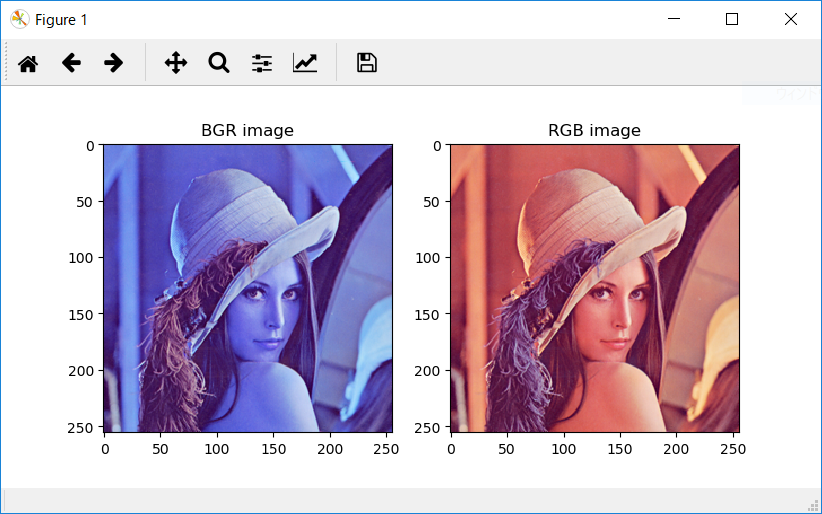
\includegraphics[width=10cm]{./figs/bgr_rgb.png}
		\end{center}
	\end{frame}
	
	\begin{frame}[fragile]{簡単な画像処理をかける例}
	    \begin{itemize}
	        \item 画像をぼかすフィルタを適用する
	        \item フィルタの設計に関する詳細は10章でやる
	    \end{itemize}
	    \scriptsize
	    \begin{minted}{python}
import cv2
from matplotlib import pyplot as plt

img_src = cv2.imread('../images/mono/BRIDGE.bmp')
assert img_src is not None, 'Loading image is failed.'

# 画像をぼかす処理をかける
img_dst = cv2.blur(img_src, (9, 9))

plt.subplot(1, 2, 1), plt.imshow(img_src), plt.title('src image')
plt.subplot(1, 2, 2), plt.imshow(img_dst), plt.title('dst image')
# plt.savefig('filename.png')
# plt.savefig('filename.pdf')
plt.show()
	    \end{minted}
	\end{frame}
	
	\begin{frame}{実行結果}
		\begin{center}
			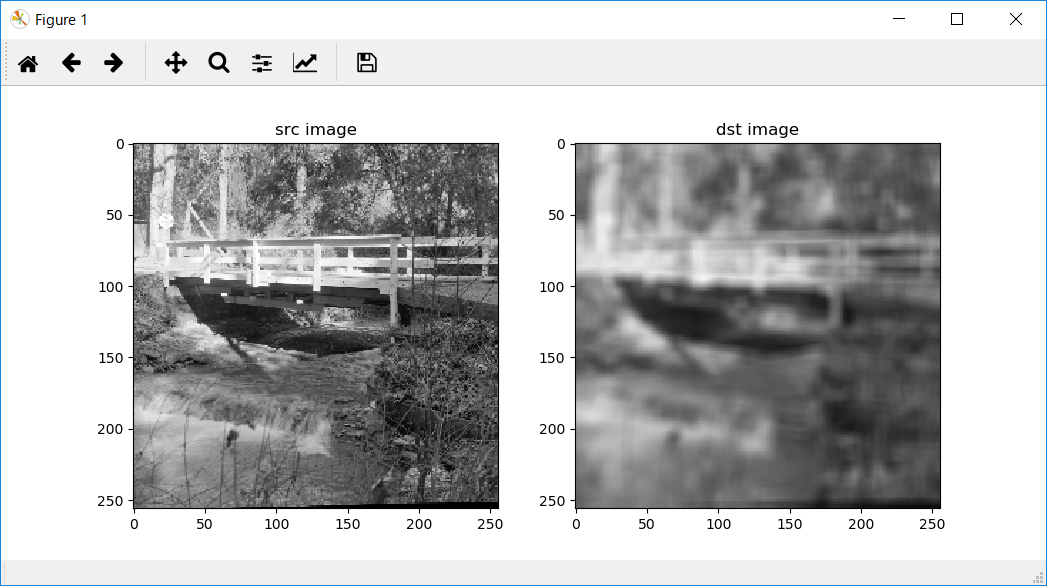
\includegraphics[width=10cm]{./figs/blur.png}
		\end{center}
	\end{frame}
	
	\begin{frame}[fragile]{動画をファイルに書き出す}
	    \tiny
	    \begin{minted}{python}
import cv2

cv2.namedWindow('Example 2-11', cv2.WINDOW_AUTOSIZE)

cap = cv2.VideoCapture(0)
assert cap.isOpened(), 'Cannot open the video.'

width = int(cap.get(cv2.CAP_PROP_FRAME_WIDTH))      # 映像の横幅を取得
height = int(cap.get(cv2.CAP_PROP_FRAME_HEIGHT))    # 映像の縦幅を取得

fps = 15.0 # FPSは動画ファイルからは自動取得できるけどカメラからは無理?

# 動画書き込みを行うクラスのインスタンスを作る
writer = cv2.VideoWriter('video.mp4', cv2.VideoWriter_fourcc(*'MJPG'), fps, (width, height))

for k in range(100):
    
    ok, frame = cap.read()
    
    if not ok:
        break
    
    cv2.imshow('Example 2-11', frame)
    writer.write(frame)
    
    key = cv2.waitKey(33)
    if key >= 0:
        break

cap.release()
writer.release()
cv2.destroyAllWindows()
	    \end{minted}
	\end{frame}
	
	\section{10章:フィルタとコンボリューション}
	
	\begin{frame}{画像フィルタリング}
		\begin{itemize}
			\item 画像を色の値からなる「2次元配列」ではなく,「2変数関数」と解釈する
			\item 画像フィルタリング:入力画像$I(x, y)$から新しい画像$I'(x, y)$を計算するアルゴリズム
				\begin{itemize}
					\item 例1:ある画像からぼけた画像を生成する
					\item 例2:ある画像を白と黒のみからなる画像に変換する
				\end{itemize}
		\end{itemize}
	\end{frame}
	
	\begin{frame}{画像フィルタリングの内容はカーネルによって定義される}
		\begin{itemize}
			\item 出力画像$I'(x, y)$の位置$(x, y)$における画素値は入力画像中の位置$(x, y)$周辺の画素から計算される
			\[ I'(x, y) = \sum_{i, j \in \mathit{kernel}} k_{i, j} \cdot I(x + i, y + j) \]
			\item 上式中の$k_{i, j}$を\mymain{線形カーネル(フィルタ)}と呼ぶ
			\item 画像に対してカーネル(線形,非線形問わず)を
				適用する操作を\mymain{コンボリューション}と呼ぶ
		\end{itemize}
	\end{frame}

	\begin{frame}{線形カーネルと適用のイメージ}
		\begin{center}
	        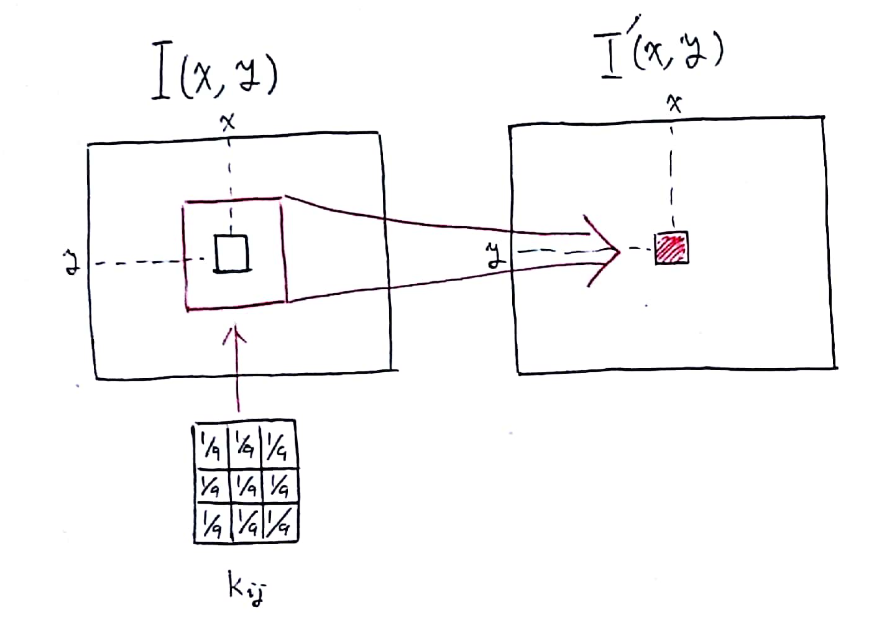
\includegraphics[width=10cm]{figs/linear_filtering.png}
	    \end{center}
	\end{frame}

	\begin{frame}[fragile]{線形カーネルによる画像フィルタリングの例:平滑化}
		\scriptsize
		\begin{minted}{python}
import cv2
from matplotlib import pyplot as plt

img_src = cv2.imread('../images/mono/BRIDGE.bmp')
assert img_src is not None, 'Loading image is failed.'

# 画像に9 x 9の平均化フィルタを適用する
img_dst = cv2.blur(img_src, (9, 9))

plt.subplot(1, 2, 1), plt.imshow(img_src), plt.title('src image')
plt.subplot(1, 2, 2), plt.imshow(img_dst), plt.title('dst image')
plt.show()
		\end{minted}
	\end{frame}
	
	\begin{frame}{実行結果}
		\begin{center}
			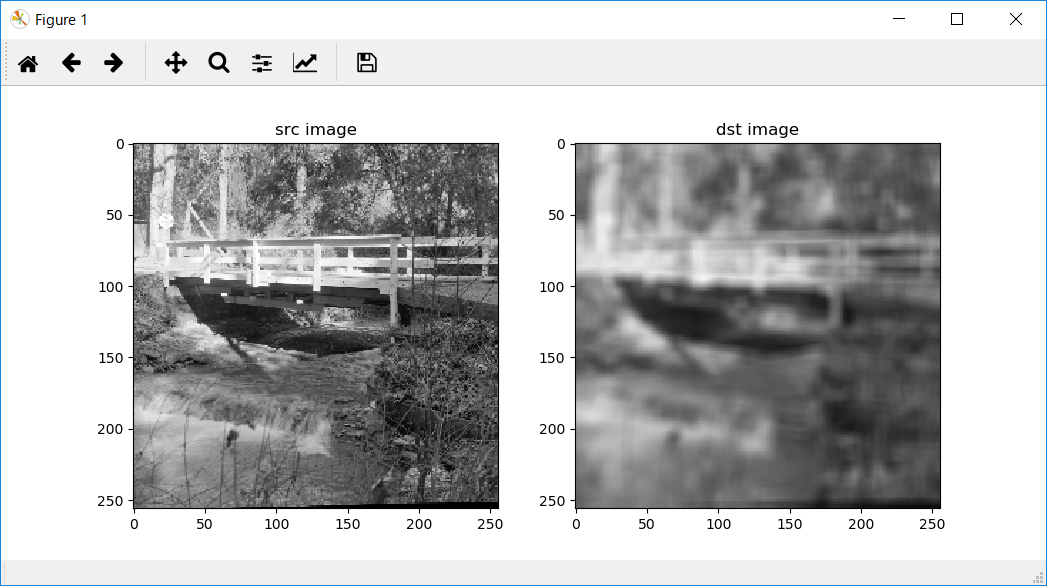
\includegraphics[width=10cm]{./figs/blur.png}
		\end{center}
	\end{frame}
	
	\begin{frame}[fragile]{閾値処理:ある値より上か下の画素を破棄する}
	    \scriptsize
		\begin{minted}{python}
# 127より明るい画素を255に,その他の画素を0にする
th, img_bin = cv2.threshold(img, 127, 255, cv2.THRESH_BINARY)
		\end{minted}
		\begin{center}
			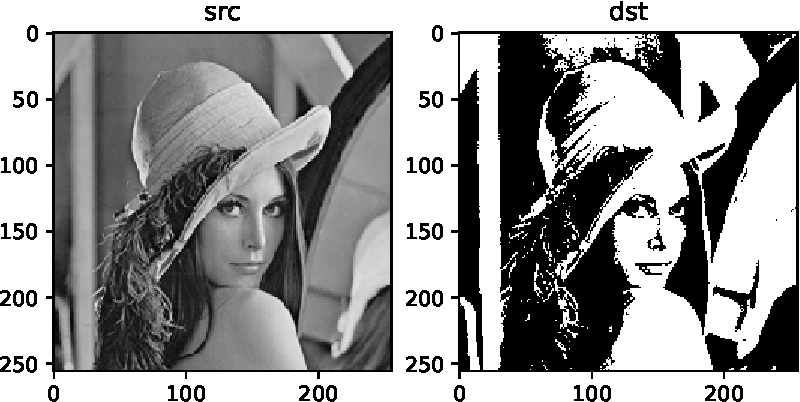
\includegraphics[width=10cm]{./figs/binary.pdf}
		\end{center}
	\end{frame}
	
	\begin{frame}{色々な閾値処理}
		\begin{itemize}
		    \item 大津の2値化
		        \item 画素が黒/白の2クラスに分類可能とみて線形判別分析をやる
		    \item 適応的閾値処理
		        \item 画像上の位置ごとに異なる閾値$T(x, y)$を設定する
                    \[ T(x, y) = \sum_{i, j \in \mathit{kernel}} k_{i, j} \cdot I(x + i, y + j) \]
                \item $k_{i,j}$はカーネル全体で等しい重みかガウス関数のどっちか
                \item 文書の画像に対する閾値処理をいい感じにできる
		\end{itemize}
	\end{frame}
	
	\begin{frame}{閾値処理の実行結果}
	    \begin{center}
			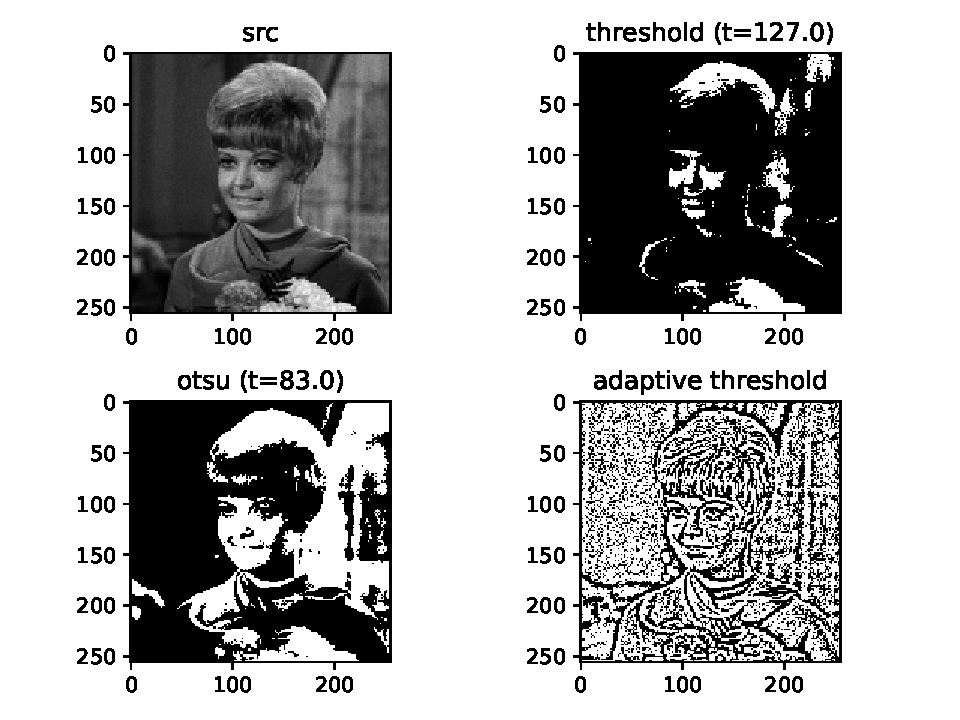
\includegraphics[width=10cm]{./figs/threshold.pdf}
		\end{center}
	\end{frame}
	
	\begin{frame}{画像の1次微分によるエッジ検出}
	    \begin{itemize}
	        \item 関数$f(x)$の微分を計算器で処理する際,
	            以下のような中心差分で近似することがある:
        	    \begin{align*}
        	        f'(x) = \lim_{\Delta x\to0}\frac{f(x+\Delta x)-f(x)}{\Delta x}
        	        \approx
        	        \frac{f(x+\Delta x)-f(x-\Delta x)}{2\Delta x}
        	    \end{align*}
        	\item ディジタル画像を扱う際は$\Delta x = 1$にとってよいので次のように書ける:
        	    \begin{align*}
        	        f'(x) = \frac{f(x+1)-f(x-1)}{2}
        	    \end{align*}
        	\item 画像$I(x, y)$は2変数関数なので,水平・垂直それぞれについて微分を定義する:
        	    \begin{align*}
        	        I_x(x, y) &= \frac{I(x+1, y)-I(x-1, y)}{2} \\
        	        I_y(x, y) &= \frac{I(x, y+1)-I(x, y-1)}{2} 
        	    \end{align*}
	    \end{itemize}
	\end{frame}
	
	\begin{frame}{画像の微分はカーネルを適用する操作として表現できる}
	    \begin{itemize}
	        \item 画像の1次微分:
        	    \begin{align*}
        	        I_x(x, y) &= \frac{I(x+1, y)-I(x-1, y)}{2} \\
        	        I_y(x, y) &= \frac{I(x, y+1)-I(x, y-1)}{2} 
        	    \end{align*}
	        \item カーネルによる表現:
        	    \begin{align*}
        	        \bm F_x = \frac{1}{2}
        	        \begin{pmatrix}
        	            0   &0  &0  \\
        	            -1   &0  &1  \\
        	            0   &0  &0  
        	        \end{pmatrix},\;\;
        	        \bm F_y = \frac{1}{2}
        	        \begin{pmatrix}
        	            0   &-1  &0  \\
        	            0   &0  &0  \\
        	            0   &1  &0  
        	        \end{pmatrix}
        	    \end{align*}
            \item ノイズの影響を抑えるために周辺画素の微分をとって
                平均を計算するフィルタ(Sobelフィルタ):
                \begin{align*}
        	        \bm F_x = \frac{1}{2}
        	        \begin{pmatrix}
        	            -1   &0  &1  \\
        	            -2   &0  &2  \\
        	            -1   &0  &1  
        	        \end{pmatrix},\;\;
        	        \bm F_y = \frac{1}{2}
        	        \begin{pmatrix}
        	            -1   &-2  &-1  \\
        	            0   &0  &0  \\
        	            1   &2  &1  
        	        \end{pmatrix}
        	    \end{align*}
	    \end{itemize}
	\end{frame}
	
	\begin{frame}{画像の2次微分:Laplacian}
	    \begin{itemize}
	        \item 連続関数$f(x, y)$のLaplacian
	            \begin{align*}
	                \nabla^2f(x,y)
	                = \frac{\partial^2f}{\partial x^2}
	                + \frac{\partial^2f}{\partial y^2}
	            \end{align*}
	        \item 画像の2次微分からLaplacianフィルタを導出する
	            \begin{align*}
	                I_{xx}(x, y) &= \{I(x + 1, y) - I(x, y)\} - \{I(x, y) - I(x-1, y)\} \\
	                             &= I(x-1,y) - 2I(x,y) + I(x+1,y) \\
	                I_{yy}(x, y) &= \{I(x, y + 1) - I(x, y)\} - \{I(x, y) - I(x, y-1)\} \\
	                             &= I(x,y-1) - 2I(x,y) + I(x,y+1) \\
	                             &\Longrightarrow
	                \bm F = 
        	        \begin{pmatrix}
        	            0   &1  &0  \\
        	            1   &-4  &1  \\
        	            0   &1  &0  
        	        \end{pmatrix}
	            \end{align*}
	    \end{itemize}
	\end{frame}
	
	\begin{frame}[fragile]{微分の実行結果}
	    \scriptsize
	    \begin{minted}{python}
sobel_x = cv2.Sobel(img, ddepth=-1, dx=1, dy=0)
sobel_y = cv2.Sobel(img, ddepth=-1, dx=0, dy=1)
img_lap = cv2.Laplacian(img, ddepth=-1, ksize=3)
	    \end{minted}
	    \begin{center}
    		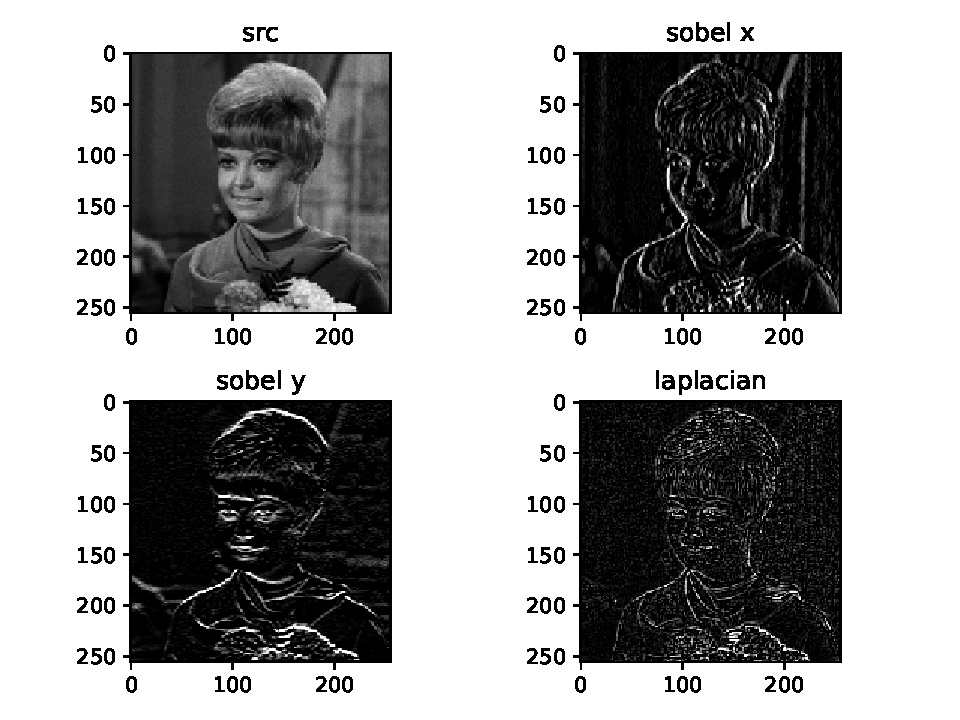
\includegraphics[width=9cm]{./figs/derivative.pdf}
		\end{center}
	\end{frame}
	
	\begin{frame}[fragile]{自前で用意した線形カーネルをたたみこむ事も可能}
	    \begin{minted}{python}
emboss = np.array([[1, 0, 0], 
                   [0, 0, 0], 
                   [0, 0,-1]])
img_emb = cv2.filter2D(img, ddepth=-1, kernel=emboss)
	    \end{minted}
	    \begin{center}
    		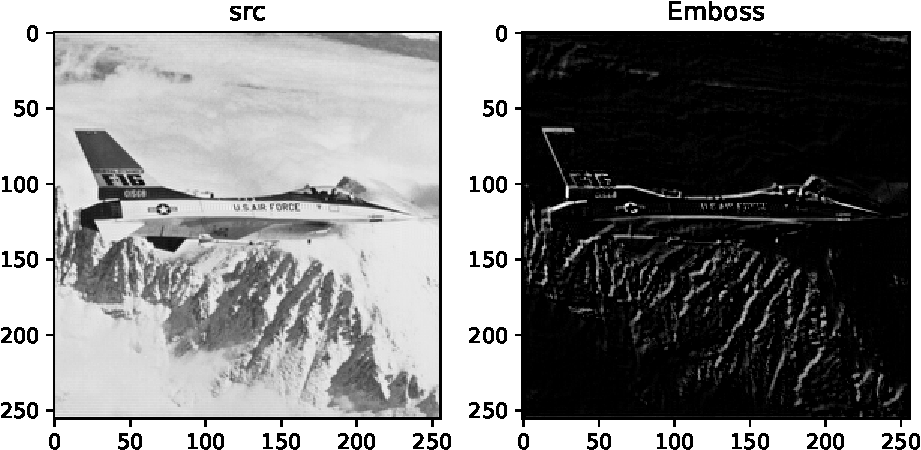
\includegraphics[width=9cm]{./figs/emboss.pdf}
		\end{center}
	\end{frame}
	
	\begin{frame}{メディアンフィルタ:エッジ保存平滑化のフィルタ}
	    \begin{itemize}
	        \item スパイクノイズ(255とか0がぽつぽつ出てくるやつ)に強い平滑化フィルタ
	        \item エッジ構造を壊さない
	    \end{itemize}
	    \begin{center}
	        スパイクノイズを重畳した画像
	        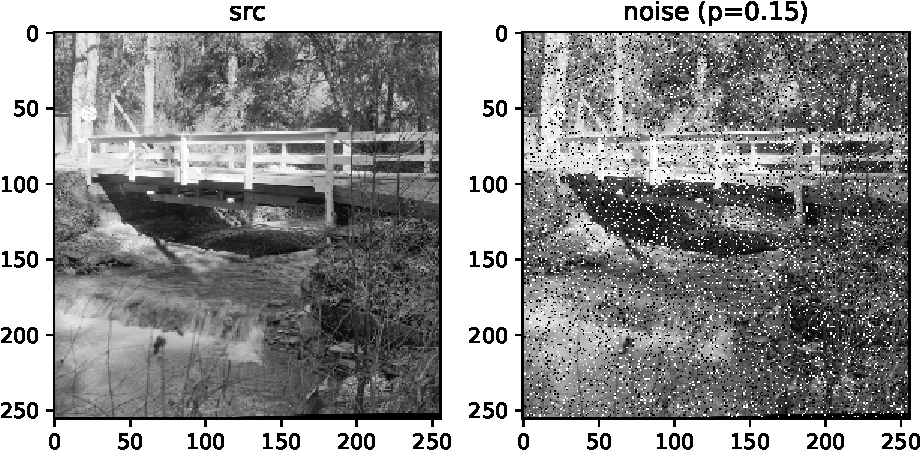
\includegraphics[width=10.0cm]{figs/spike.pdf}
	    \end{center}
	\end{frame}
	
	\begin{frame}{メディアンフィルタでは,注目領域の中央値 (メディアン) を出力の画素値とする}
	    \begin{center}
	        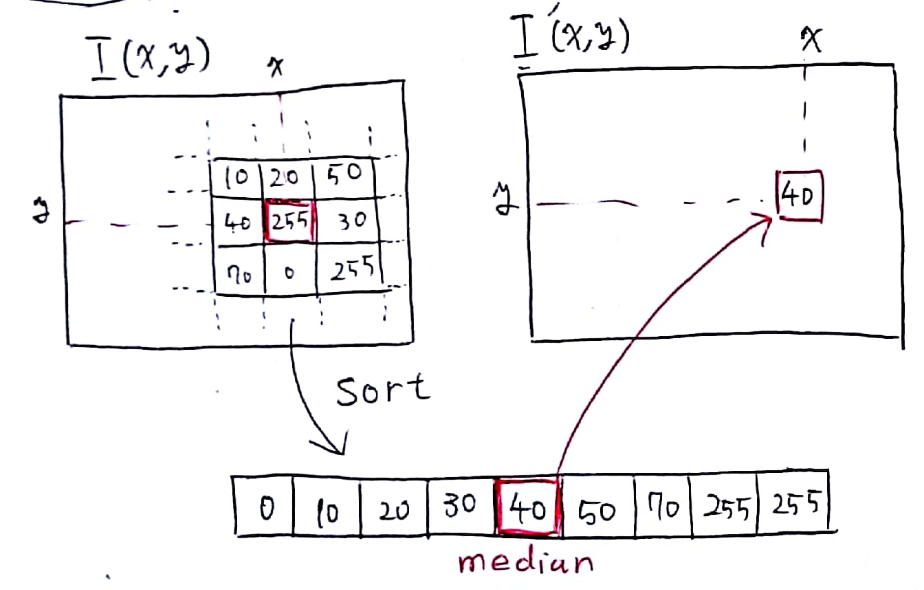
\includegraphics[width=9.0cm]{figs/median_filter.png}
	    \end{center}
	\end{frame}
	
	\begin{frame}[fragile]{スパイクノイズの重畳}
	    \scriptsize
	    \begin{minted}{python}
def apply_noise(img, p=0.05):
    """ 画像にノイズを重畳する関数 """

    # 画素数
    npixels = img.size
    random_indices = np.random.permutation(npixels)
    # ノイズが重畳される画素のインデックス
    salt_idx   = random_indices[:int(npixels*p/2.0)]
    pepper_idx = random_indices[int(npixels*p/2.0):int(npixels*p)]
    # 画像をフラットにした配列を取得
    img_flat = img.flatten()
    img_flat[salt_idx] = 255
    img_flat[pepper_idx] = 0

    return img_flat.reshape(img.shape)
	    \end{minted}
	    \begin{tikzpicture}[overlay, remember picture]
            \node[above left=1cm and .8cm of current page.south east] {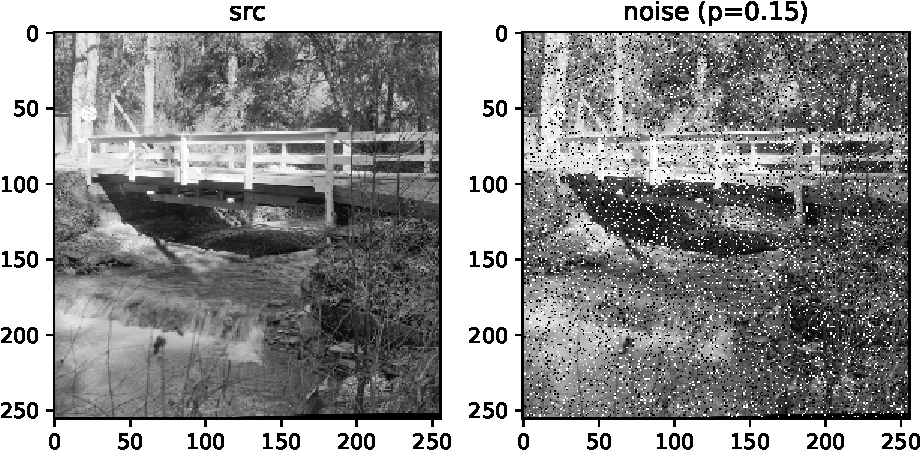
\includegraphics[width=5.0cm]{figs/spike.pdf}};
        \end{tikzpicture}
	\end{frame}
	
	\begin{frame}[fragile]{メディアンフィルタの実行結果}
	    \begin{minted}[fontsize=\scriptsize]{python}
img_median = cv2.medianBlur(img, 5)
	    \end{minted}
	    \vspace{-0.25cm}\\
	    \begin{center}
	        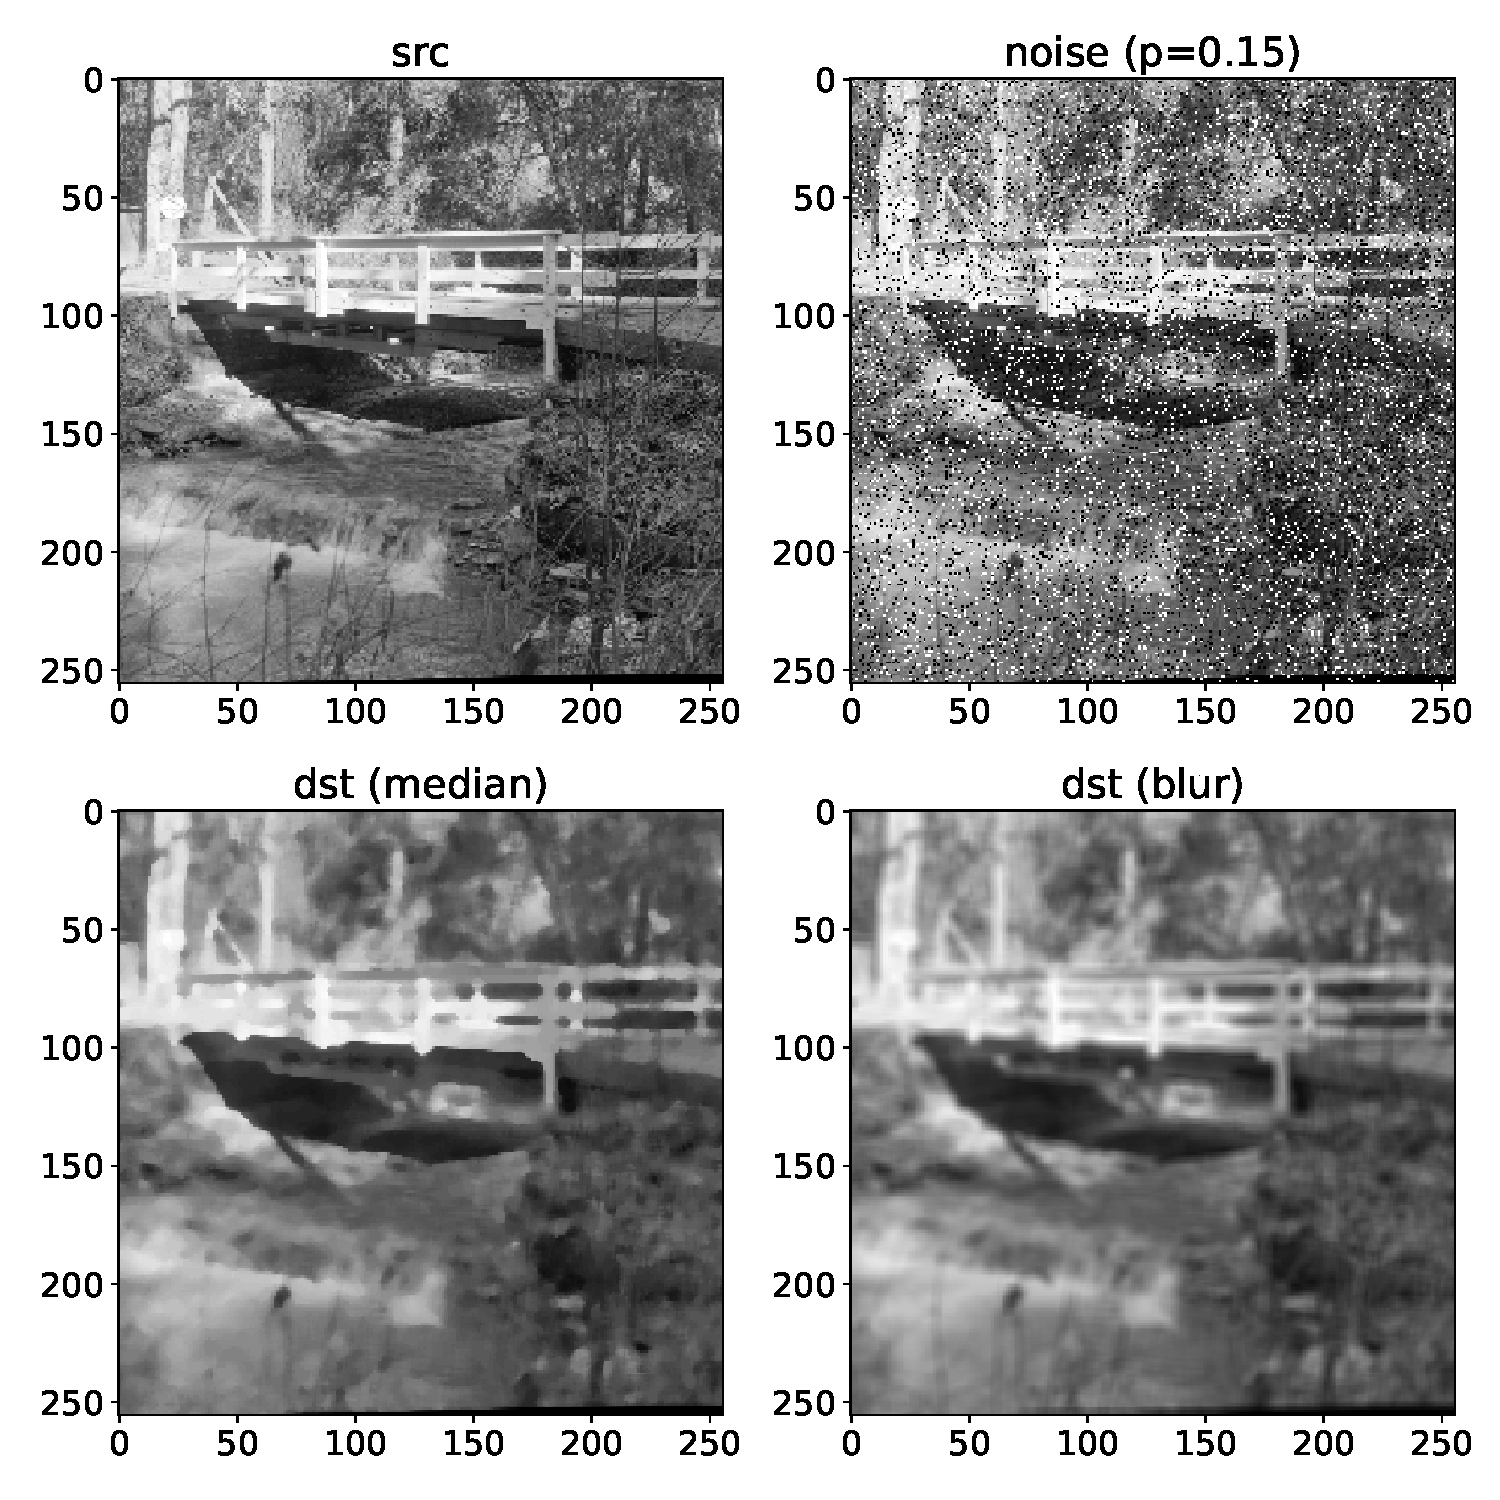
\includegraphics[width=7.5cm]{figs/median.pdf}
	    \end{center}
	\end{frame}
	
	\begin{frame}{モルフォロジー変換:\\膨張 (dilation) と収縮 (erosion) を基本演算とする演算方法}
	    \begin{columns}
	        \begin{column}[c]{0.3\hsize}\centering
	            元画像\par
    	        
\includegraphics[width=0.9\hsize]{figs/morph_src.png}
	        \end{column}
	        \begin{column}[c]{0.3\hsize}\centering
	            膨張\par
    	        
\includegraphics[width=0.9\hsize]{figs/dilation.png}
	        \end{column}
	        \begin{column}[c]{0.3\hsize}\centering
	            収縮 \par
    	        
\includegraphics[width=0.9\hsize]{figs/erosion.png}
	        \end{column}
	    \end{columns}
	\end{frame}
	
	\begin{frame}{モルフォロジー変換の基本演算はメディアンフィルタに似てる}
	    \begin{center}
	        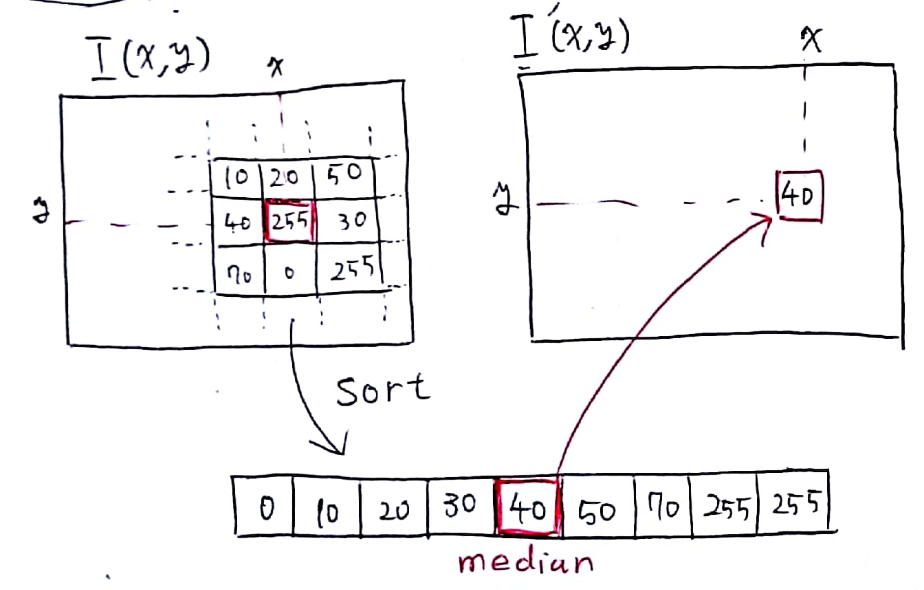
\includegraphics[width=7.0cm]{figs/median_filter.png}
	    \end{center}
	    \begin{itemize}
	        \item 膨張:メディアンフィルタのmedianをmaxに置き換えたもの
	        \item 収縮:メディアンフィルタのmedianをminに置き換えたもの
	        \item 一般のグレースケール画像についても定義されるが,
	            2値画像に対して適用する例が多い
	    \end{itemize}
	\end{frame}
	
	\begin{frame}{膨張と収縮を組み合わせた演算の例}
	    \begin{columns}
	        \begin{column}[c]{0.5\hsize}\centering
	            Opening \par
    	        
\includegraphics[width=0.9\hsize]{figs/opening.png}
	        \end{column}
	        \begin{column}[c]{0.5\hsize}\centering
	            Closing \par
    	        
\includegraphics[width=0.9\hsize]{figs/closing.png}
	        \end{column}
	    \end{columns}
	    \begin{itemize}
	        \item Opening: 収縮してから膨張する
	            \begin{itemize}
	                \item 2値画像中の孤立のノイズを消せる
	            \end{itemize}
	        \item Closing: 膨張してから収縮する
	            \begin{itemize}
	                \item 2値画像中の図形中の小さい穴を消せる
	            \end{itemize}
	    \end{itemize}
	\end{frame}
	
	\begin{frame}[fragile]{モルフォロジー変換の構造化要素 (Structuring Element)}
	    \begin{itemize}
	        \item モルフォロジー変換のカーネルの形状を定義するもの
	        \item 矩形の範囲だけでなく,円形や棒状の範囲でのモルフォロジー変換を作ることができる
	    \end{itemize}
	    \begin{minted}[fontsize=\scriptsize]{python}
>>> cv.getStructuringElement(cv.MORPH_RECT, (5, 5))
array([[1, 1, 1, 1, 1],
       [1, 1, 1, 1, 1],
       [1, 1, 1, 1, 1],
       [1, 1, 1, 1, 1],
       [1, 1, 1, 1, 1]], dtype=uint8)

>>> cv.getStructuringElement(cv.MORPH_ELLIPSE, (5, 5))
array([[0, 0, 1, 0, 0],
       [1, 1, 1, 1, 1],
       [1, 1, 1, 1, 1],
       [1, 1, 1, 1, 1],
       [0, 0, 1, 0, 0]], dtype=uint8)
	    \end{minted}
	\end{frame}
	
	\section{13章:ヒストグラムとテンプレートマッチング}
	
	\begin{frame}{マッチング:2つの画像が同じかどうかを判断する問題}
	    \begin{itemize}
	        \item 問題の例
        	    \begin{itemize}
        	        \item 回路基板の画像から特定の素子を探したい
        	        \item ハンドジェスチャの種類を判定
        	    \end{itemize}
	        \item 2つのアプローチが紹介されている
        	    \begin{itemize}
        	        \item 画素や勾配方向のヒストグラムのマッチング
        	        \item 画像の類似度によるマッチング
        	    \end{itemize}
        	\item デモ: {\tiny \url{https://docs.opencv.org/3.4/d8/dd1/tutorial_js_template_matching.html}}
	    \end{itemize}
	\end{frame}
	
	\begin{frame}{画素値のヒストグラムを計算する}
	    \begin{center}
	        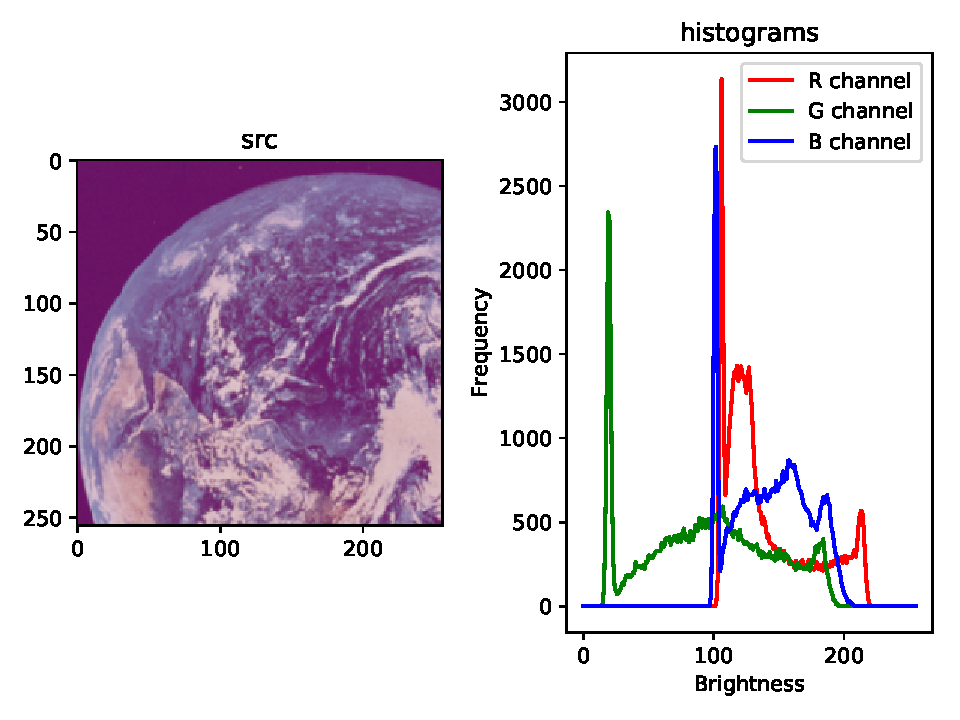
\includegraphics[width=0.7\hsize]{figs/compute_hist.pdf}
	    \end{center}
	    \begin{itemize}
	        \item R--G間のBhattacharyya距離: 0.630
	        \item R--B間のBhattacharyya距離: 0.428
	        \item G--B間のBhattacharyya距離: 0.574
	    \end{itemize}
	\end{frame}
	
	\begin{frame}{画像のヒストグラムはOpenCVの機能でもNumpyの機能でも計算できる}
	    \begin{center}
	        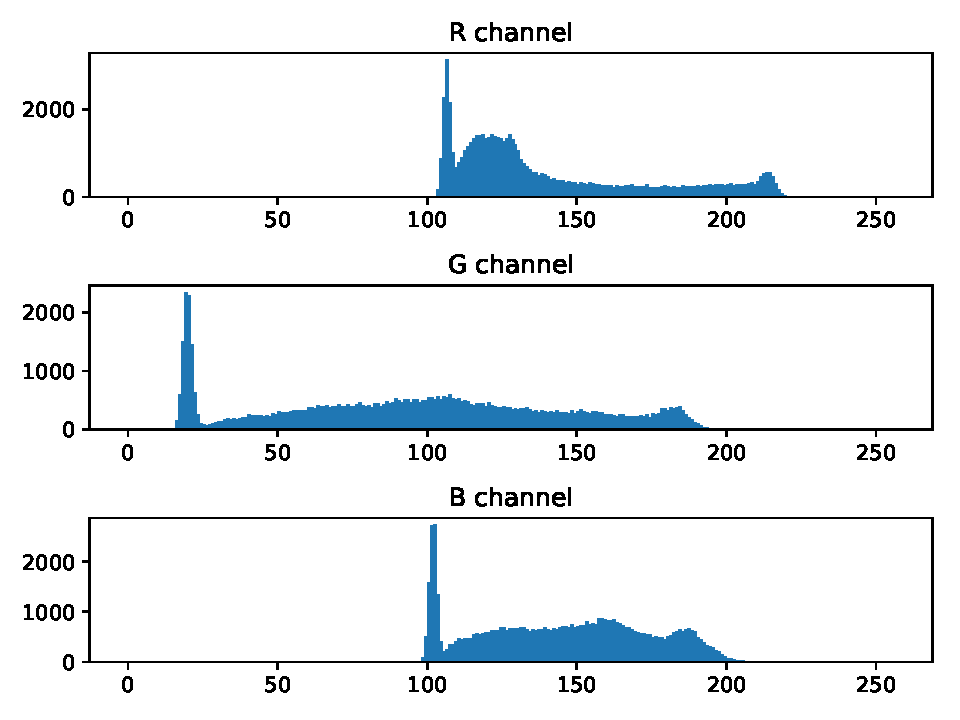
\includegraphics[width=0.8\hsize]{figs/compute_hist_numpy.pdf}
	    \end{center}
	\end{frame}
	
	\begin{frame}{テンプレートマッチング}
	    \begin{itemize}
	        \item 入力画像からテンプレート画像と類似する部分を探す方法
	    \end{itemize}
	    \begin{center}
	        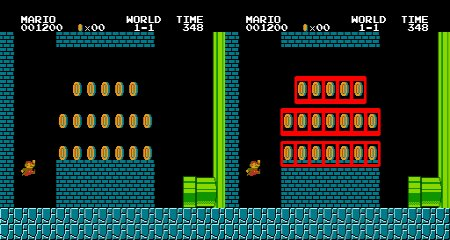
\includegraphics[width=0.9\hsize]{figs/res_mario.jpg}
	    \end{center}
	\end{frame}
	
	\begin{frame}{画像$I(x, y)$とテンプレート画像$T(x, y)$間の類似度を測る方法}
	    \begin{itemize}
	        \item 二乗差分マッチング手法 (\texttt{cv2.TM\_SQDIFF})
	            \begin{itemize}
	                \item 完全一致は0.不一致は大きい値になる.
	            \end{itemize}
	            \[
	                R = \sum_{x',y'} \left[ T(x',y') - I(x+x', y+y') \right]^2
	            \]
	        \item 正規化二乗差分マッチング手法 (\texttt{cv2.TM\_SQDIFF\_NORMED})
	            \begin{itemize}
	                \item 完全一致は0.
	            \end{itemize}
	        \item 相互相関マッチング手法 (\texttt{cv2.TM\_CCORR})
	            \begin{itemize}
	                \item 一致すると大きな値,不一致は小さな値になり,最小値は0
	            \end{itemize}
	            \[
	                R = \sum_{x',y'}T(x',y')\cdot I(x+x', y+y')
	            \]
	    \end{itemize}
	\end{frame}
	
	\begin{frame}{テンプレートマッチング}
	    \begin{center}
	        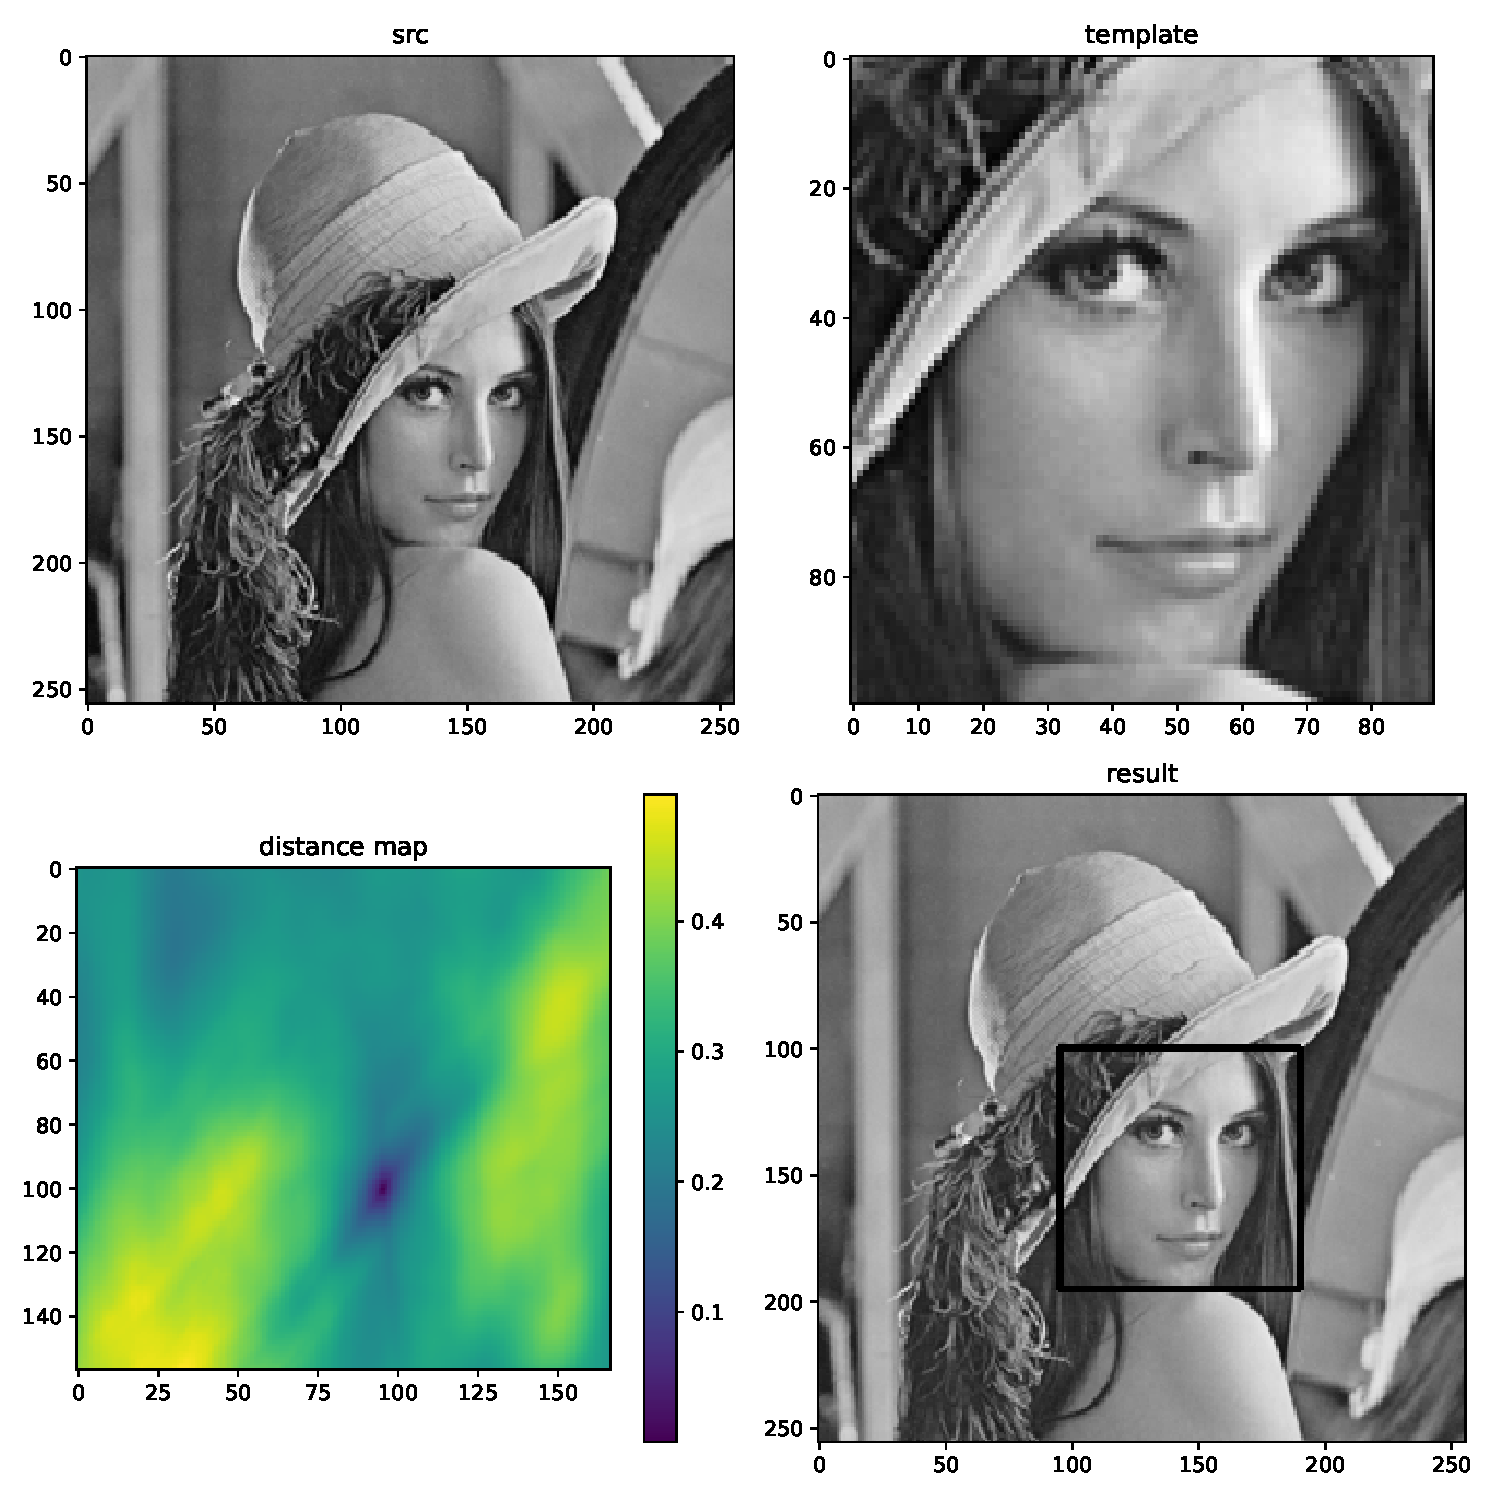
\includegraphics[width=0.7\hsize]{figs/template_matching.pdf}
	    \end{center}
	\end{frame}
	
	\section{14章:輪郭}
	
	\begin{frame}{輪郭検出: 点の集合で輪郭を表現する}
	    \begin{itemize}
	        \item LaplacianやCannyエッジ検出器はエッジを検出してもその形状の情報は与えてくれない
	    \end{itemize}
	\end{frame}
	
	\begin{frame}{輪郭を囲む矩形を計算する}
	    \begin{itemize}
	        \item \texttt{cv2.boundingRect()}
	        \item \texttt{cv2.minAreaRect()}
	    \end{itemize}
	\end{frame}
	
	\begin{frame}{輪郭を囲む楕円形を計算する}
	    \begin{itemize}
	        \item \texttt{cv2.minEnclosingCircle()}
	        \item \texttt{cv2.fitEllipse()}
	    \end{itemize}
	\end{frame}
	
	\begin{frame}{モーメントによる輪郭の比較}
	    
	\end{frame}
	
	\begin{frame}{演習:マウスの動画解析}
	    \begin{center}
	        \url{https://bit.ly/2GiMNPA}
	    \end{center}
	    今まで学習した内容でどこまでできそう?
	    \begin{enumerate}
	        \item マウスの体の中心位置を追跡
	            \begin{itemize}
	                \item 簡単そう
	            \end{itemize}
	        \item マウスの体の向きを追跡
	            \begin{itemize}
	                \item 尻尾の位置がわかれば体の中心位置との組み合わせでいけそう
	            \end{itemize}
	        \item マウスの頭の向きを追跡
	            \begin{itemize}
	                \item 頭は体の向きと独立に動くので難しそう
	            \end{itemize}
	    \end{enumerate}
	\end{frame}
	
	\if0
		\begin{frame}{LoG: Laplacian of Gaussianフィルタ}
	    \begin{itemize}
	        \item Laplacianフィルタはノイズを拾いやすいので,
	            ガウシアンフィルタ$G(x,y,\sigma)$による平滑化をしてからLaplacianを計算することがある
	            \begin{align*}
	                \nabla^2(G(x,y,\sigma)\ast I(x,y)) = (\nabla^2G(x,y,\sigma)) \ast I(x,y)
	            \end{align*}
	        \item $\nabla^2G(x,y,\sigma)$をLaplacian of Gaussian (LoG) フィルタという
	        \item 平滑化の強さは$\sigma$をいじることで調整可能
	    \end{itemize}
	\end{frame}
	\fi
	
	\if0
	\section{12章:画像解析}
	
	\begin{frame}{画像の周波数解析}
	    \begin{itemize}
	        \item 今回はスキップします
	        \item 画像の離散Fourier変換や離散コサイン変換の話
	        \item JPEGみたいな画像圧縮に興味があるならやるといいかも
	    \end{itemize}
	\end{frame}
	
	\begin{frame}{Cannyエッジ検出器}
	    
	\end{frame}
	
	\begin{frame}{Cannyエッジ検出器の原理}
	    
	\end{frame}
	
	\begin{frame}{直線のHough変換}
	    
	\end{frame}
	
	\begin{frame}{距離変換}

	\end{frame}
	
	\begin{frame}{平均値シフト:画像の領域分割}
	    
	\end{frame}
	\fi

\end{document}
